%Author: Simon Dorrer, k12005887
%% !TeX document-id = {b8e7f259-21c3-4834-b29d-9cf620be8d99}
%% !BIB program = biber
\documentclass[12pt, twoside]{report}

%Language Settings:
\usepackage[utf8]{inputenc}
\usepackage[english]{babel}
\usepackage[T1]{fontenc}		%Separation pattern

\usepackage{geometry}

\usepackage{fancyhdr}

%Text generation
\usepackage{lipsum}	

%Tables
\usepackage{numprint}
\usepackage{longtable}						%Table over several pages
\usepackage[table]{xcolor}

%Pictures
\usepackage{float}
\usepackage{graphicx}

%Verweise
\usepackage{url}
\usepackage{hyperref}

%Math
\usepackage{amsmath}
\usepackage{amssymb}

\usepackage[nottoc]{tocbibind}

%Bibliography
%\usepackage{biblatex}
%\addbibresource{bibliography.bib}

% Acronyms
\usepackage{acronym}

%PDF Pages
\usepackage{pdfpages}

%Adding Arduino Language
 %%%%%%%%%%%%%%%%%%%%%%%%%%%%%%%%%%%%%%%%%%%%%%%%%%%%%%%%%%%%%%%%%%%%%%%%%%%%%%%% 
%%% ~ Arduino Language - Arduino IDE Colors ~                                  %%%
%%%                                                                            %%%
%%% Kyle Rocha-Brownell | 10/2/2017 | No Licence                               %%%
%%% -------------------------------------------------------------------------- %%%
%%%                                                                            %%%
%%% Place this file in your working directory (next to the latex file you're   %%%
%%% working on).  To add it to your project, place:                            %%%
%%%     %%%%%%%%%%%%%%%%%%%%%%%%%%%%%%%%%%%%%%%%%%%%%%%%%%%%%%%%%%%%%%%%%%%%%%%%%%%%%%%% 
%%% ~ Arduino Language - Arduino IDE Colors ~                                  %%%
%%%                                                                            %%%
%%% Kyle Rocha-Brownell | 10/2/2017 | No Licence                               %%%
%%% -------------------------------------------------------------------------- %%%
%%%                                                                            %%%
%%% Place this file in your working directory (next to the latex file you're   %%%
%%% working on).  To add it to your project, place:                            %%%
%%%    \input{arduinoLanguage.tex}                                             %%%
%%% somewhere before \begin{document} in your latex file.                      %%%
%%%                                                                            %%%
%%% In your document, place your arduino code between:                         %%%
%%%   \begin{lstlisting}[language=Arduino]                                     %%%
%%% and:                                                                       %%%
%%%   \end{lstlisting}                                                         %%%
%%%                                                                            %%%
%%% Or create your own style to add non-built-in functions and variables.      %%%
%%%                                                                            %%%
%%%%%%%%%%%%%%%%%%%%%%%%%%%%%%%%%%%%%%%%%%%%%%%%%%%%%%%%%%%%%%%%%%%%%%%%%%%%%%%% 

\usepackage{color}
\usepackage{listings}    
\usepackage{courier}

%%% Define Custom IDE Colors %%%
\definecolor{arduinoGreen}    {rgb} {0.17, 0.43, 0.01}
\definecolor{arduinoGrey}     {rgb} {0.47, 0.47, 0.33}
\definecolor{arduinoOrange}   {rgb} {0.8 , 0.4 , 0   }
\definecolor{arduinoBlue}     {rgb} {0.01, 0.61, 0.98}
\definecolor{arduinoDarkBlue} {rgb} {0.0 , 0.2 , 0.5 }

%%% Define Arduino Language %%%
\lstdefinelanguage{Arduino}{
	language=C++, % begin with default C++ settings 
	%
	%
	%%% Keyword Color Group 1 %%%  (called KEYWORD3 by arduino)
	keywordstyle=\color{arduinoGreen},   
	deletekeywords={  % remove all arduino keywords that might be in c++
		break, case, override, final, continue, default, do, else, for, 
		if, return, goto, switch, throw, try, while, setup, loop, export, 
		not, or, and, xor, include, define, elif, else, error, if, ifdef, 
		ifndef, pragma, warning,
		HIGH, LOW, INPUT, INPUT_PULLUP, OUTPUT, DEC, BIN, HEX, OCT, PI, 
		HALF_PI, TWO_PI, LSBFIRST, MSBFIRST, CHANGE, FALLING, RISING, 
		DEFAULT, EXTERNAL, INTERNAL, INTERNAL1V1, INTERNAL2V56, LED_BUILTIN, 
		LED_BUILTIN_RX, LED_BUILTIN_TX, DIGITAL_MESSAGE, FIRMATA_STRING, 
		ANALOG_MESSAGE, REPORT_DIGITAL, REPORT_ANALOG, SET_PIN_MODE, 
		SYSTEM_RESET, SYSEX_START, auto, int8_t, int16_t, int32_t, int64_t, 
		uint8_t, uint16_t, uint32_t, uint64_t, char16_t, char32_t, operator, 
		enum, delete, bool, boolean, byte, char, const, false, float, double, 
		null, NULL, int, long, new, private, protected, public, short, 
		signed, static, volatile, String, void, true, unsigned, word, array, 
		sizeof, dynamic_cast, typedef, const_cast, struct, static_cast, union, 
		friend, extern, class, reinterpret_cast, register, explicit, inline, 
		_Bool, complex, _Complex, _Imaginary, atomic_bool, atomic_char, 
		atomic_schar, atomic_uchar, atomic_short, atomic_ushort, atomic_int, 
		atomic_uint, atomic_long, atomic_ulong, atomic_llong, atomic_ullong, 
		virtual, PROGMEM,
		Serial, Serial1, Serial2, Serial3, SerialUSB, Keyboard, Mouse,
		abs, acos, asin, atan, atan2, ceil, constrain, cos, degrees, exp, 
		floor, log, map, max, min, radians, random, randomSeed, round, sin, 
		sq, sqrt, tan, pow, bitRead, bitWrite, bitSet, bitClear, bit, 
		highByte, lowByte, analogReference, analogRead, 
		analogReadResolution, analogWrite, analogWriteResolution, 
		attachInterrupt, detachInterrupt, digitalPinToInterrupt, delay, 
		delayMicroseconds, digitalWrite, digitalRead, interrupts, millis, 
		micros, noInterrupts, noTone, pinMode, pulseIn, pulseInLong, shiftIn, 
		shiftOut, tone, yield, Stream, begin, end, peek, read, print, 
		println, available, availableForWrite, flush, setTimeout, find, 
		findUntil, parseInt, parseFloat, readBytes, readBytesUntil, readString, 
		readStringUntil, trim, toUpperCase, toLowerCase, charAt, compareTo, 
		concat, endsWith, startsWith, equals, equalsIgnoreCase, getBytes, 
		indexOf, lastIndexOf, length, replace, setCharAt, substring, 
		toCharArray, toInt, press, release, releaseAll, accept, click, move, 
		isPressed, isAlphaNumeric, isAlpha, isAscii, isWhitespace, isControl, 
		isDigit, isGraph, isLowerCase, isPrintable, isPunct, isSpace, 
		isUpperCase, isHexadecimalDigit, 
	}, 
	morekeywords={   % add arduino structures to group 1
		break, case, override, final, continue, default, do, else, for, 
		if, return, goto, switch, throw, try, while, setup, loop, export, 
		not, or, and, xor, include, define, elif, else, error, if, ifdef, 
		ifndef, pragma, warning,
	}, 
	% 
	%
	%%% Keyword Color Group 2 %%%  (called LITERAL1 by arduino)
	keywordstyle=[2]\color{arduinoBlue},   
	keywords=[2]{   % add variables and dataTypes as 2nd group  
		HIGH, LOW, INPUT, INPUT_PULLUP, OUTPUT, DEC, BIN, HEX, OCT, PI, 
		HALF_PI, TWO_PI, LSBFIRST, MSBFIRST, CHANGE, FALLING, RISING, 
		DEFAULT, EXTERNAL, INTERNAL, INTERNAL1V1, INTERNAL2V56, LED_BUILTIN, 
		LED_BUILTIN_RX, LED_BUILTIN_TX, DIGITAL_MESSAGE, FIRMATA_STRING, 
		ANALOG_MESSAGE, REPORT_DIGITAL, REPORT_ANALOG, SET_PIN_MODE, 
		SYSTEM_RESET, SYSEX_START, auto, int8_t, int16_t, int32_t, int64_t, 
		uint8_t, uint16_t, uint32_t, uint64_t, char16_t, char32_t, operator, 
		enum, delete, bool, boolean, byte, char, const, false, float, double, 
		null, NULL, int, long, new, private, protected, public, short, 
		signed, static, volatile, String, void, true, unsigned, word, array, 
		sizeof, dynamic_cast, typedef, const_cast, struct, static_cast, union, 
		friend, extern, class, reinterpret_cast, register, explicit, inline, 
		_Bool, complex, _Complex, _Imaginary, atomic_bool, atomic_char, 
		atomic_schar, atomic_uchar, atomic_short, atomic_ushort, atomic_int, 
		atomic_uint, atomic_long, atomic_ulong, atomic_llong, atomic_ullong, 
		virtual, PROGMEM,
	},  
	% 
	%
	%%% Keyword Color Group 3 %%%  (called KEYWORD1 by arduino)
	keywordstyle=[3]\bfseries\color{arduinoOrange},
	keywords=[3]{  % add built-in functions as a 3rd group
		Serial, Serial1, Serial2, Serial3, SerialUSB, Keyboard, Mouse,
	},      
	%
	%
	%%% Keyword Color Group 4 %%%  (called KEYWORD2 by arduino)
	keywordstyle=[4]\color{arduinoOrange},
	keywords=[4]{  % add more built-in functions as a 4th group
		abs, acos, asin, atan, atan2, ceil, constrain, cos, degrees, exp, 
		floor, log, map, max, min, radians, random, randomSeed, round, sin, 
		sq, sqrt, tan, pow, bitRead, bitWrite, bitSet, bitClear, bit, 
		highByte, lowByte, analogReference, analogRead, 
		analogReadResolution, analogWrite, analogWriteResolution, 
		attachInterrupt, detachInterrupt, digitalPinToInterrupt, delay, 
		delayMicroseconds, digitalWrite, digitalRead, interrupts, millis, 
		micros, noInterrupts, noTone, pinMode, pulseIn, pulseInLong, shiftIn, 
		shiftOut, tone, yield, Stream, begin, end, peek, read, print, 
		println, available, availableForWrite, flush, setTimeout, find, 
		findUntil, parseInt, parseFloat, readBytes, readBytesUntil, readString, 
		readStringUntil, trim, toUpperCase, toLowerCase, charAt, compareTo, 
		concat, endsWith, startsWith, equals, equalsIgnoreCase, getBytes, 
		indexOf, lastIndexOf, length, replace, setCharAt, substring, 
		toCharArray, toInt, press, release, releaseAll, accept, click, move, 
		isPressed, isAlphaNumeric, isAlpha, isAscii, isWhitespace, isControl, 
		isDigit, isGraph, isLowerCase, isPrintable, isPunct, isSpace, 
		isUpperCase, isHexadecimalDigit, 
	},      
	%
	%
	%%% Set Other Colors %%%
	stringstyle=\color{arduinoDarkBlue},    
	commentstyle=\color{arduinoGrey},    
	%          
	%   
	%%%% Line Numbering %%%%
	numbers=left,                    
	numbersep=5pt,                   
	numberstyle=\color{arduinoGrey},    
	%stepnumber=2,                      % show every 2 line numbers
	%
	%
	%%%% Code Box Style %%%%
	breaklines=true,                    % wordwrapping
	tabsize=2,         
	basicstyle=\ttfamily  
}                                             %%%
%%% somewhere before \begin{document} in your latex file.                      %%%
%%%                                                                            %%%
%%% In your document, place your arduino code between:                         %%%
%%%   \begin{lstlisting}[language=Arduino]                                     %%%
%%% and:                                                                       %%%
%%%   \end{lstlisting}                                                         %%%
%%%                                                                            %%%
%%% Or create your own style to add non-built-in functions and variables.      %%%
%%%                                                                            %%%
%%%%%%%%%%%%%%%%%%%%%%%%%%%%%%%%%%%%%%%%%%%%%%%%%%%%%%%%%%%%%%%%%%%%%%%%%%%%%%%% 

\usepackage{color}
\usepackage{listings}    
\usepackage{courier}

%%% Define Custom IDE Colors %%%
\definecolor{arduinoGreen}    {rgb} {0.17, 0.43, 0.01}
\definecolor{arduinoGrey}     {rgb} {0.47, 0.47, 0.33}
\definecolor{arduinoOrange}   {rgb} {0.8 , 0.4 , 0   }
\definecolor{arduinoBlue}     {rgb} {0.01, 0.61, 0.98}
\definecolor{arduinoDarkBlue} {rgb} {0.0 , 0.2 , 0.5 }

%%% Define Arduino Language %%%
\lstdefinelanguage{Arduino}{
	language=C++, % begin with default C++ settings 
	%
	%
	%%% Keyword Color Group 1 %%%  (called KEYWORD3 by arduino)
	keywordstyle=\color{arduinoGreen},   
	deletekeywords={  % remove all arduino keywords that might be in c++
		break, case, override, final, continue, default, do, else, for, 
		if, return, goto, switch, throw, try, while, setup, loop, export, 
		not, or, and, xor, include, define, elif, else, error, if, ifdef, 
		ifndef, pragma, warning,
		HIGH, LOW, INPUT, INPUT_PULLUP, OUTPUT, DEC, BIN, HEX, OCT, PI, 
		HALF_PI, TWO_PI, LSBFIRST, MSBFIRST, CHANGE, FALLING, RISING, 
		DEFAULT, EXTERNAL, INTERNAL, INTERNAL1V1, INTERNAL2V56, LED_BUILTIN, 
		LED_BUILTIN_RX, LED_BUILTIN_TX, DIGITAL_MESSAGE, FIRMATA_STRING, 
		ANALOG_MESSAGE, REPORT_DIGITAL, REPORT_ANALOG, SET_PIN_MODE, 
		SYSTEM_RESET, SYSEX_START, auto, int8_t, int16_t, int32_t, int64_t, 
		uint8_t, uint16_t, uint32_t, uint64_t, char16_t, char32_t, operator, 
		enum, delete, bool, boolean, byte, char, const, false, float, double, 
		null, NULL, int, long, new, private, protected, public, short, 
		signed, static, volatile, String, void, true, unsigned, word, array, 
		sizeof, dynamic_cast, typedef, const_cast, struct, static_cast, union, 
		friend, extern, class, reinterpret_cast, register, explicit, inline, 
		_Bool, complex, _Complex, _Imaginary, atomic_bool, atomic_char, 
		atomic_schar, atomic_uchar, atomic_short, atomic_ushort, atomic_int, 
		atomic_uint, atomic_long, atomic_ulong, atomic_llong, atomic_ullong, 
		virtual, PROGMEM,
		Serial, Serial1, Serial2, Serial3, SerialUSB, Keyboard, Mouse,
		abs, acos, asin, atan, atan2, ceil, constrain, cos, degrees, exp, 
		floor, log, map, max, min, radians, random, randomSeed, round, sin, 
		sq, sqrt, tan, pow, bitRead, bitWrite, bitSet, bitClear, bit, 
		highByte, lowByte, analogReference, analogRead, 
		analogReadResolution, analogWrite, analogWriteResolution, 
		attachInterrupt, detachInterrupt, digitalPinToInterrupt, delay, 
		delayMicroseconds, digitalWrite, digitalRead, interrupts, millis, 
		micros, noInterrupts, noTone, pinMode, pulseIn, pulseInLong, shiftIn, 
		shiftOut, tone, yield, Stream, begin, end, peek, read, print, 
		println, available, availableForWrite, flush, setTimeout, find, 
		findUntil, parseInt, parseFloat, readBytes, readBytesUntil, readString, 
		readStringUntil, trim, toUpperCase, toLowerCase, charAt, compareTo, 
		concat, endsWith, startsWith, equals, equalsIgnoreCase, getBytes, 
		indexOf, lastIndexOf, length, replace, setCharAt, substring, 
		toCharArray, toInt, press, release, releaseAll, accept, click, move, 
		isPressed, isAlphaNumeric, isAlpha, isAscii, isWhitespace, isControl, 
		isDigit, isGraph, isLowerCase, isPrintable, isPunct, isSpace, 
		isUpperCase, isHexadecimalDigit, 
	}, 
	morekeywords={   % add arduino structures to group 1
		break, case, override, final, continue, default, do, else, for, 
		if, return, goto, switch, throw, try, while, setup, loop, export, 
		not, or, and, xor, include, define, elif, else, error, if, ifdef, 
		ifndef, pragma, warning,
	}, 
	% 
	%
	%%% Keyword Color Group 2 %%%  (called LITERAL1 by arduino)
	keywordstyle=[2]\color{arduinoBlue},   
	keywords=[2]{   % add variables and dataTypes as 2nd group  
		HIGH, LOW, INPUT, INPUT_PULLUP, OUTPUT, DEC, BIN, HEX, OCT, PI, 
		HALF_PI, TWO_PI, LSBFIRST, MSBFIRST, CHANGE, FALLING, RISING, 
		DEFAULT, EXTERNAL, INTERNAL, INTERNAL1V1, INTERNAL2V56, LED_BUILTIN, 
		LED_BUILTIN_RX, LED_BUILTIN_TX, DIGITAL_MESSAGE, FIRMATA_STRING, 
		ANALOG_MESSAGE, REPORT_DIGITAL, REPORT_ANALOG, SET_PIN_MODE, 
		SYSTEM_RESET, SYSEX_START, auto, int8_t, int16_t, int32_t, int64_t, 
		uint8_t, uint16_t, uint32_t, uint64_t, char16_t, char32_t, operator, 
		enum, delete, bool, boolean, byte, char, const, false, float, double, 
		null, NULL, int, long, new, private, protected, public, short, 
		signed, static, volatile, String, void, true, unsigned, word, array, 
		sizeof, dynamic_cast, typedef, const_cast, struct, static_cast, union, 
		friend, extern, class, reinterpret_cast, register, explicit, inline, 
		_Bool, complex, _Complex, _Imaginary, atomic_bool, atomic_char, 
		atomic_schar, atomic_uchar, atomic_short, atomic_ushort, atomic_int, 
		atomic_uint, atomic_long, atomic_ulong, atomic_llong, atomic_ullong, 
		virtual, PROGMEM,
	},  
	% 
	%
	%%% Keyword Color Group 3 %%%  (called KEYWORD1 by arduino)
	keywordstyle=[3]\bfseries\color{arduinoOrange},
	keywords=[3]{  % add built-in functions as a 3rd group
		Serial, Serial1, Serial2, Serial3, SerialUSB, Keyboard, Mouse,
	},      
	%
	%
	%%% Keyword Color Group 4 %%%  (called KEYWORD2 by arduino)
	keywordstyle=[4]\color{arduinoOrange},
	keywords=[4]{  % add more built-in functions as a 4th group
		abs, acos, asin, atan, atan2, ceil, constrain, cos, degrees, exp, 
		floor, log, map, max, min, radians, random, randomSeed, round, sin, 
		sq, sqrt, tan, pow, bitRead, bitWrite, bitSet, bitClear, bit, 
		highByte, lowByte, analogReference, analogRead, 
		analogReadResolution, analogWrite, analogWriteResolution, 
		attachInterrupt, detachInterrupt, digitalPinToInterrupt, delay, 
		delayMicroseconds, digitalWrite, digitalRead, interrupts, millis, 
		micros, noInterrupts, noTone, pinMode, pulseIn, pulseInLong, shiftIn, 
		shiftOut, tone, yield, Stream, begin, end, peek, read, print, 
		println, available, availableForWrite, flush, setTimeout, find, 
		findUntil, parseInt, parseFloat, readBytes, readBytesUntil, readString, 
		readStringUntil, trim, toUpperCase, toLowerCase, charAt, compareTo, 
		concat, endsWith, startsWith, equals, equalsIgnoreCase, getBytes, 
		indexOf, lastIndexOf, length, replace, setCharAt, substring, 
		toCharArray, toInt, press, release, releaseAll, accept, click, move, 
		isPressed, isAlphaNumeric, isAlpha, isAscii, isWhitespace, isControl, 
		isDigit, isGraph, isLowerCase, isPrintable, isPunct, isSpace, 
		isUpperCase, isHexadecimalDigit, 
	},      
	%
	%
	%%% Set Other Colors %%%
	stringstyle=\color{arduinoDarkBlue},    
	commentstyle=\color{arduinoGrey},    
	%          
	%   
	%%%% Line Numbering %%%%
	numbers=left,                    
	numbersep=5pt,                   
	numberstyle=\color{arduinoGrey},    
	%stepnumber=2,                      % show every 2 line numbers
	%
	%
	%%%% Code Box Style %%%%
	breaklines=true,                    % wordwrapping
	tabsize=2,         
	basicstyle=\ttfamily  
}
%Geometry of document: A4 portrait
%\geometry{paper=a4paper, top=1.6cm, bottom=2.85cm, left=0.9cm, right=2.15cm}
%\geometry{paper=a4paper, top=3.6cm, bottom=3.6cm, left=2.6cm, right=3.7cm}
\geometry{paper = a4paper, left = 20mm, right = 15mm, top = 15mm, bottom = 12.5mm, includeheadfoot}

%Header formation
\pagestyle{fancy}
\fancyhf{}												% Clear header / footer
\fancyhead[EL, OR]{\textsc{\nouppercase{\leftmark}}}    % Chapter in the right on even pages
\fancyhead[ER, OL]{\thepage}							%Page number location
\fancyfoot[ER, OL]{\copyright\/ Simon Dorrer, OE3SDE}	%Copyright + Name + Matrikelnmmer

\fancypagestyle{plain}{									%set pagestyle also for plain page
	\pagestyle{fancy}
}

%Separation line header / footer with 1.25pt
%\renewcommand{\headrulewidth}{1.25pt}
%\renewcommand{\footrulewidth}{1.25pt}

% Optional: Correct bad hyphenation
\hyphenation{}

%10mm area between header / footer and textarea
\setlength{\headsep}{10mm}
\setlength{\footskip}{12.5mm}

%No indentation, 1.1ex between paragraphs
\setlength{\parindent}{0ex}
\setlength{\parskip}{1.1ex plus0.25ex minus0.25ex}
%Title
\title{\emph{60W 144MHz FM Power Amplifier}}	%Set title (no new page)
\author{by Simon Dorrer, OE3SDE}				%Set Name and matrikelnumber (also \footnote instead of \thanks is possible)
\date{\today}									%Set date

\begin{document}
	% Align text on top if there is space left on the page (no rubber lengths will be stretched)
	\raggedbottom
	\maketitle
	
	% Abstract
	\begin{abstract}
	This 60W 144MHz FM Power Amplifier is the perfect "Add-On" for my previously released 1W 144MHz FM Transceiver. This power amplifier adds 30dB gain in the TX-Path and a lot of important analog RF filtering. Furthermore, the RX-Path is amplified with a gain of 23dB and is filtered with high order filters to improve the signal noise ration for better understanding of the other transmitters.
	All RX / TX signals are switched with PIN diodes to avoid expensive radio frequency shielded relais.
\end{abstract}



	\tableofcontents
	
	% -- Chapter 1 ------------------------------------------------------------------------------------	
	\chapter{Overview}
	\label{chp:overview}
	\section{Description}
On the following pages the most important details for the 60W 144MHz FM power amplifier are shown. This document includes circuits, PCB-Designs, bill of material, microcontroller codes, measurements and final result pictures.

\section{Software}
The theoretical work like circuit simulation, PCB Design and Microcontroller (MCU) programming was done with following software:
\begin{itemize}
	\item Multisim \& LTSpice: Circuit Simulation
	\item ELSIE: Analog Filter Design
	\item Autodesk EAGLE: Circuit- \& PCB-Design
	\item Autodesk Fusion 360: 3D Design
	\item Arduino: MCU Code
\end{itemize}
\newpage
\section{Devices}
The practical work like PCB assembly, fault finding and measurements are done with the following devices:
\begin{itemize}
	\item FLUKE 179 True RMS Multimeter
	\item Weller WT2020M Soldering Station
	\item Zhongdi ZD-939L Hot Air Rework Station
	\item Andonstar AD407 Digital Microscope
	\item Siglent SDS2352X-E Oscilloscope (2xCH, 350MHz)
	\item Siglent SDG2042X Function Generator (2xCH, 120MHz - hacked)
	\item Siglent SVA1015X Spektrum \& Vector Network Analyser (1.5GHz)
	\item Siglent SPD3303X-E Power Supply (2x0-32V with 3.2A, 1x2.5V/3.3V/5V with 3.2A)
	\item QJ3005EIII 300W Power Supply (2x0-30V with 5A, 1x5V with 3A)
	\item Anycubic i3 Mega S 3D Printer
\end{itemize}
A complete list of all my labor equipment can be found here: \url{https://www.oe3sde.com/Workstation.html}
	
	% -- Chapter 2 ------------------------------------------------------------------------------------	
	\chapter{Circuit}
	\label{chp:circuit}
	\section{Filters}
In ham radio applications it is very important, that transmitted signals are only in the licensed band. This power amplifier works for the 2m band, that means a frequency range of 144MHz to 146MHz.
Of course, also the received signals should be filtered to avoid any unwanted noise.
\subsection{Air Coil Calculation}
The air coils for the TX-OUT and RX-IN filters according to circuit \ref{fig:TX-OUT Filter_Circuit} and \ref{fig:RX-IN Filter_Circuit} can be calculated with the following formula:
\begin{equation}
	L = \frac{N^{2} \cdot d^{2}}{18 \cdot d + 40 \cdot l}
\end{equation}
 Where:
\begin{itemize}
	\item L = Inductance
	\item N = Number of turns
	\item d = Coil outside diameter
	\item l = Length of the coil
\end{itemize}

\bigskip
For a faster result, also an online calculator\footnote{\url{https://m0ukd.com/calculators/air-cored-inductor-calculator/}} \cite{airCoilCalculator.2015} can be used. 

\newpage
\subsection{TX-IN Filter}
This filter is build up with SMT components because of the low input power of 0.5W.
The TX-IN filter is a seventh order chebyshev low pass filter with a cutoff frequency of 175MHz.
The high order is chosen because of the high harmonic distortion of the DRA818V \acs{TRX} at the input.
\begin{figure}[ht!]
	\centering
	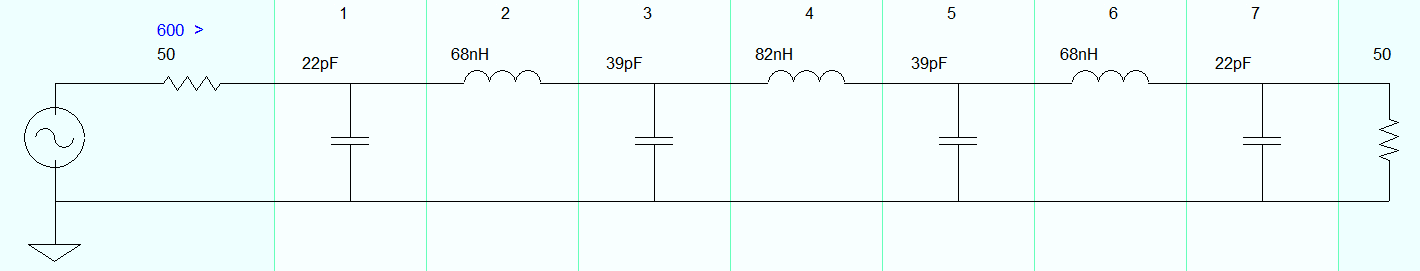
\includegraphics[width = 17cm]{./2_circuit/fig/TX-IN Filter_Circuit}
	\caption{Circuit of the TX-IN Filter}
	\label{fig:TX-IN Filter_Circuit}
\end{figure}
\bigskip
\begin{figure}[ht!]
	\centering
	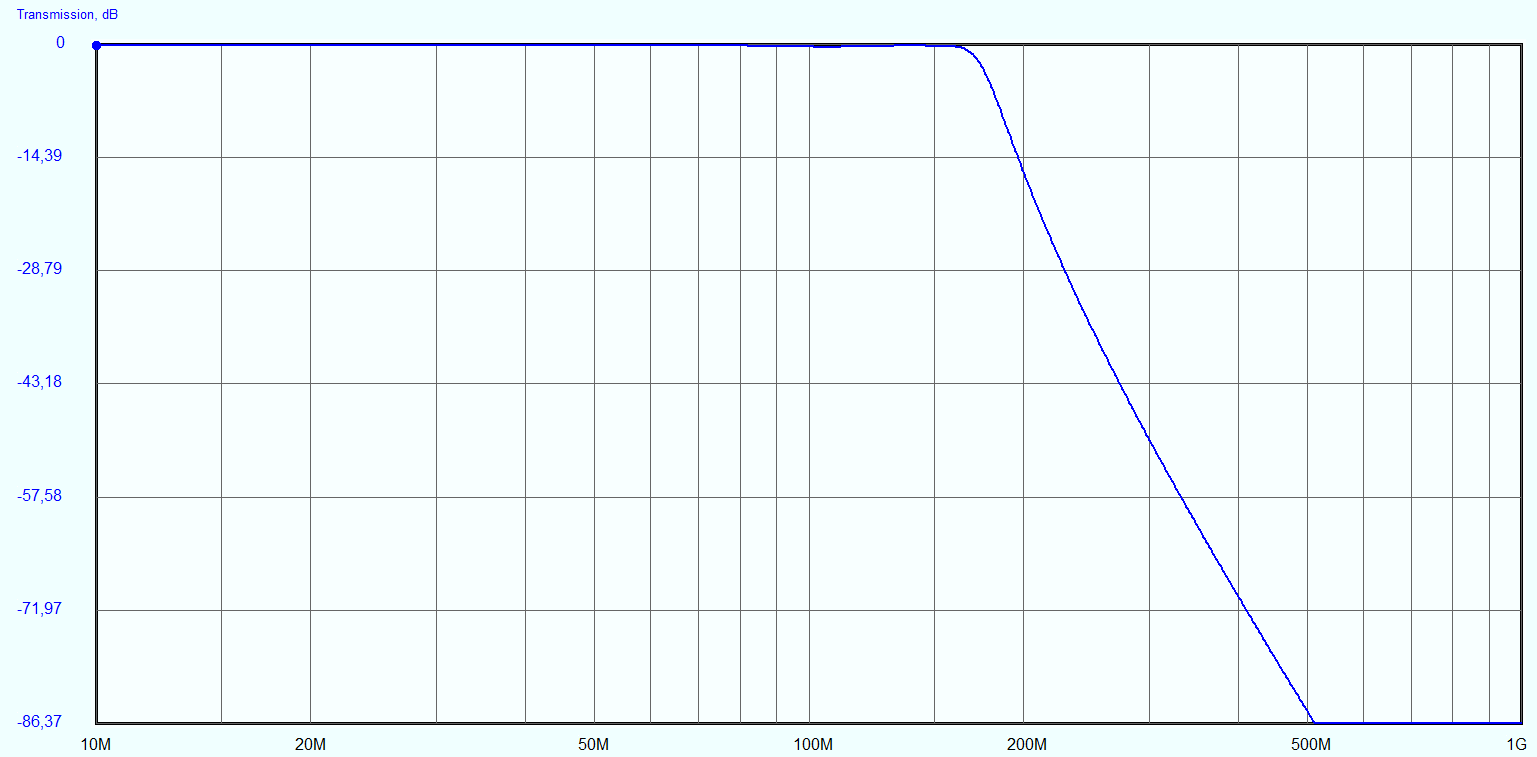
\includegraphics[width = 17cm]{./2_circuit/fig/TX-IN Filter_TF}
	\caption{Transfer Function of the TX-IN Filter}
	\label{fig:TX-IN Filter_TF}
\end{figure}

\newpage
\subsection{TX-OUT Filter}
This filter is build up with self-wound inductors because of the higher output power of 60W.
The TX-OUT filter is a fifth order chebyshev low pass filter with a cutoff frequency of 182MHz.

\begin{figure}[ht!]
	\centering
	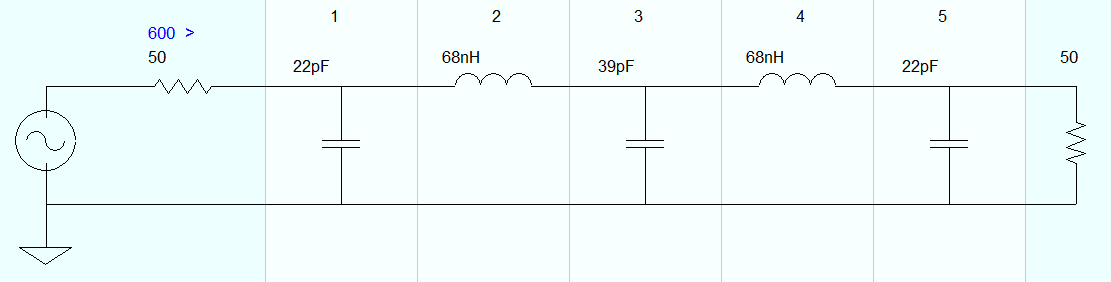
\includegraphics[width = 17cm]{./2_circuit/fig/TX-OUT Filter_Circuit}
	\caption{Circuit of the TX-OUT Filter}
	\label{fig:TX-OUT Filter_Circuit}
\end{figure}
\bigskip
\begin{figure}[ht!]
	\centering
	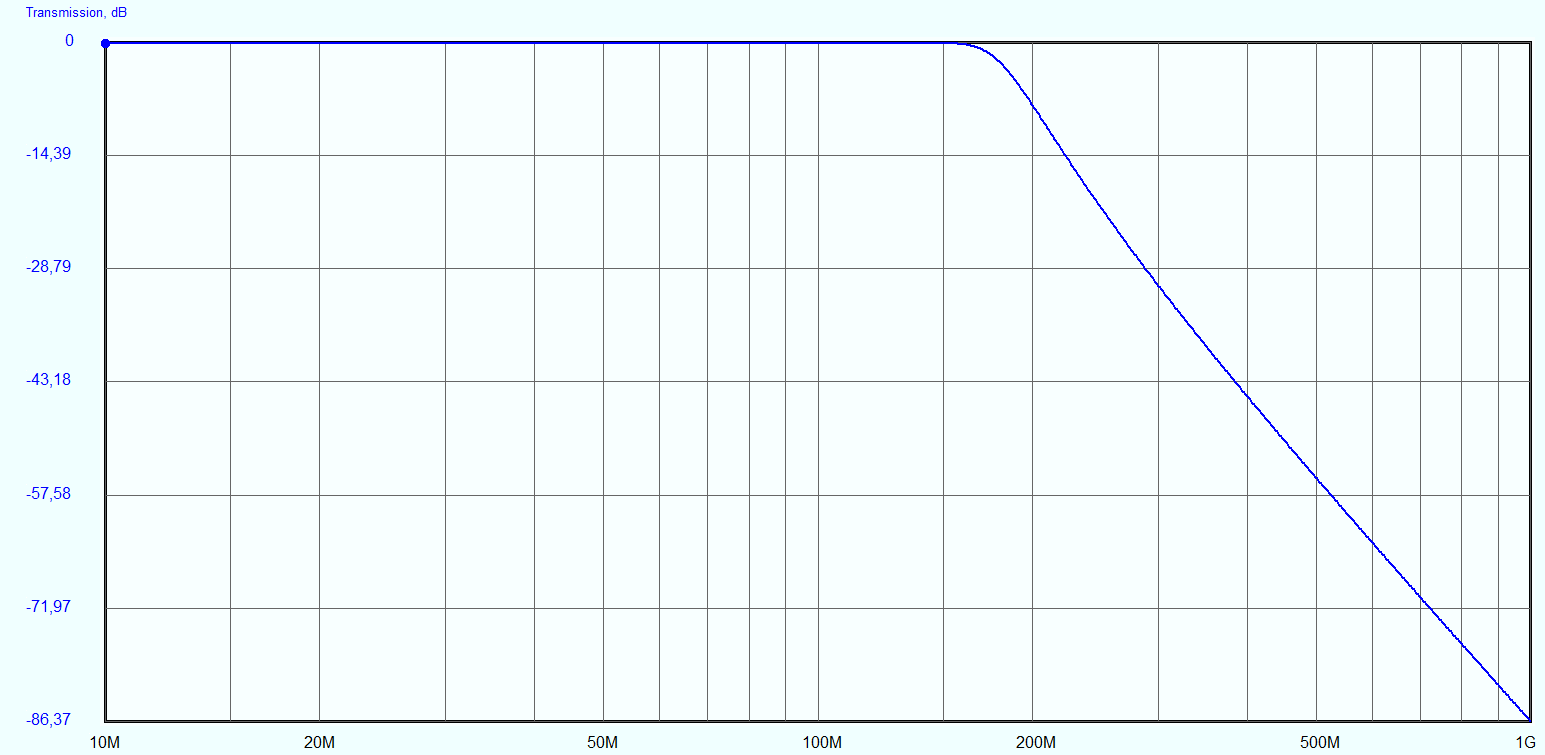
\includegraphics[width = 17cm]{./2_circuit/fig/TX-OUT Filter_TF}
	\caption{Transfer Function of the TX-OUT Filter}
	\label{fig:TX-OUT Filter_TF}
\end{figure}

\newpage
\subsection{RX-IN Filter}
This filter can be build up with SMT components. However, self-wound inductors can be changed easier and the filter band can be adjusted slightly.
The RX-IN filter is a third order chebyshev band pass filter with a lower cutoff frequency of 120MHz and a upper cutoff frequency of 172MHz.

\begin{figure}[ht!]
	\centering
	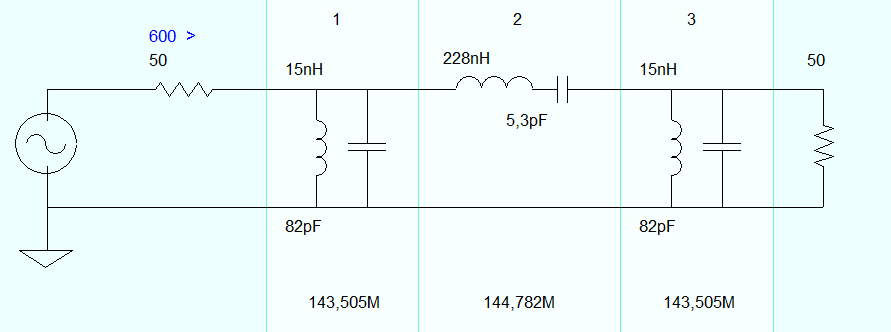
\includegraphics[width = 17cm]{./2_circuit/fig/RX-IN Filter_Circuit}
	\caption{Circuit of the RX-IN Filter}
	\label{fig:RX-IN Filter_Circuit}
\end{figure}
\bigskip
\begin{figure}[ht!]
	\centering
	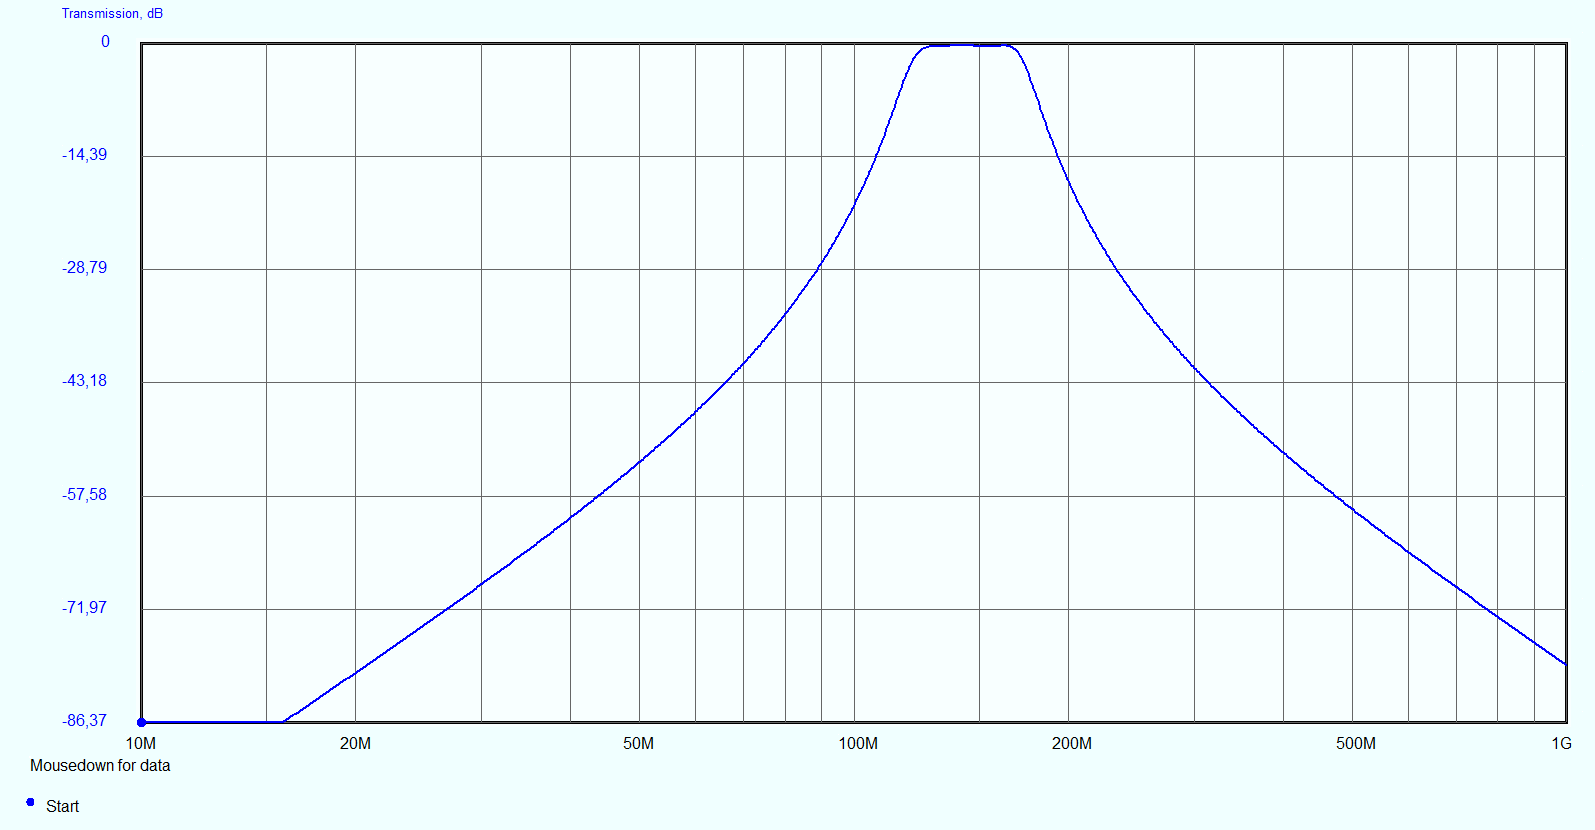
\includegraphics[width = 17cm]{./2_circuit/fig/RX-IN Filter_TF}
	\caption{Transfer Function of the RX-IN Filter}
	\label{fig:RX-IN Filter_TF}
\end{figure}

\newpage
\section{PIN-Diode Switches}
In this project, PIN-Diodes are used instead of relais to switch between RX and TX path.
\subsection{RX/TX Input-Switch}
ToDo Text
\begin{figure}[ht!]
	\centering
	%\includegraphics[width = 12cm]{./2_circuit/fig/}
	\includegraphics[width = 12cm]{example-image}
	\caption{Circuit of the RX/TX Input-Switch}
	\label{fig:RX/TX Input-Switch}
\end{figure}

\newpage
\subsection{RX/TX Output-Switch}
ToDo Text
\begin{figure}[ht!]
	\centering
	%\includegraphics[width = 12cm]{./2_circuit/fig/}
	\includegraphics[width = 12cm]{example-image}
	\caption{Circuit of the RX/TX Output-Switch}
	\label{fig:RX/TX Output-Switch}
\end{figure}
	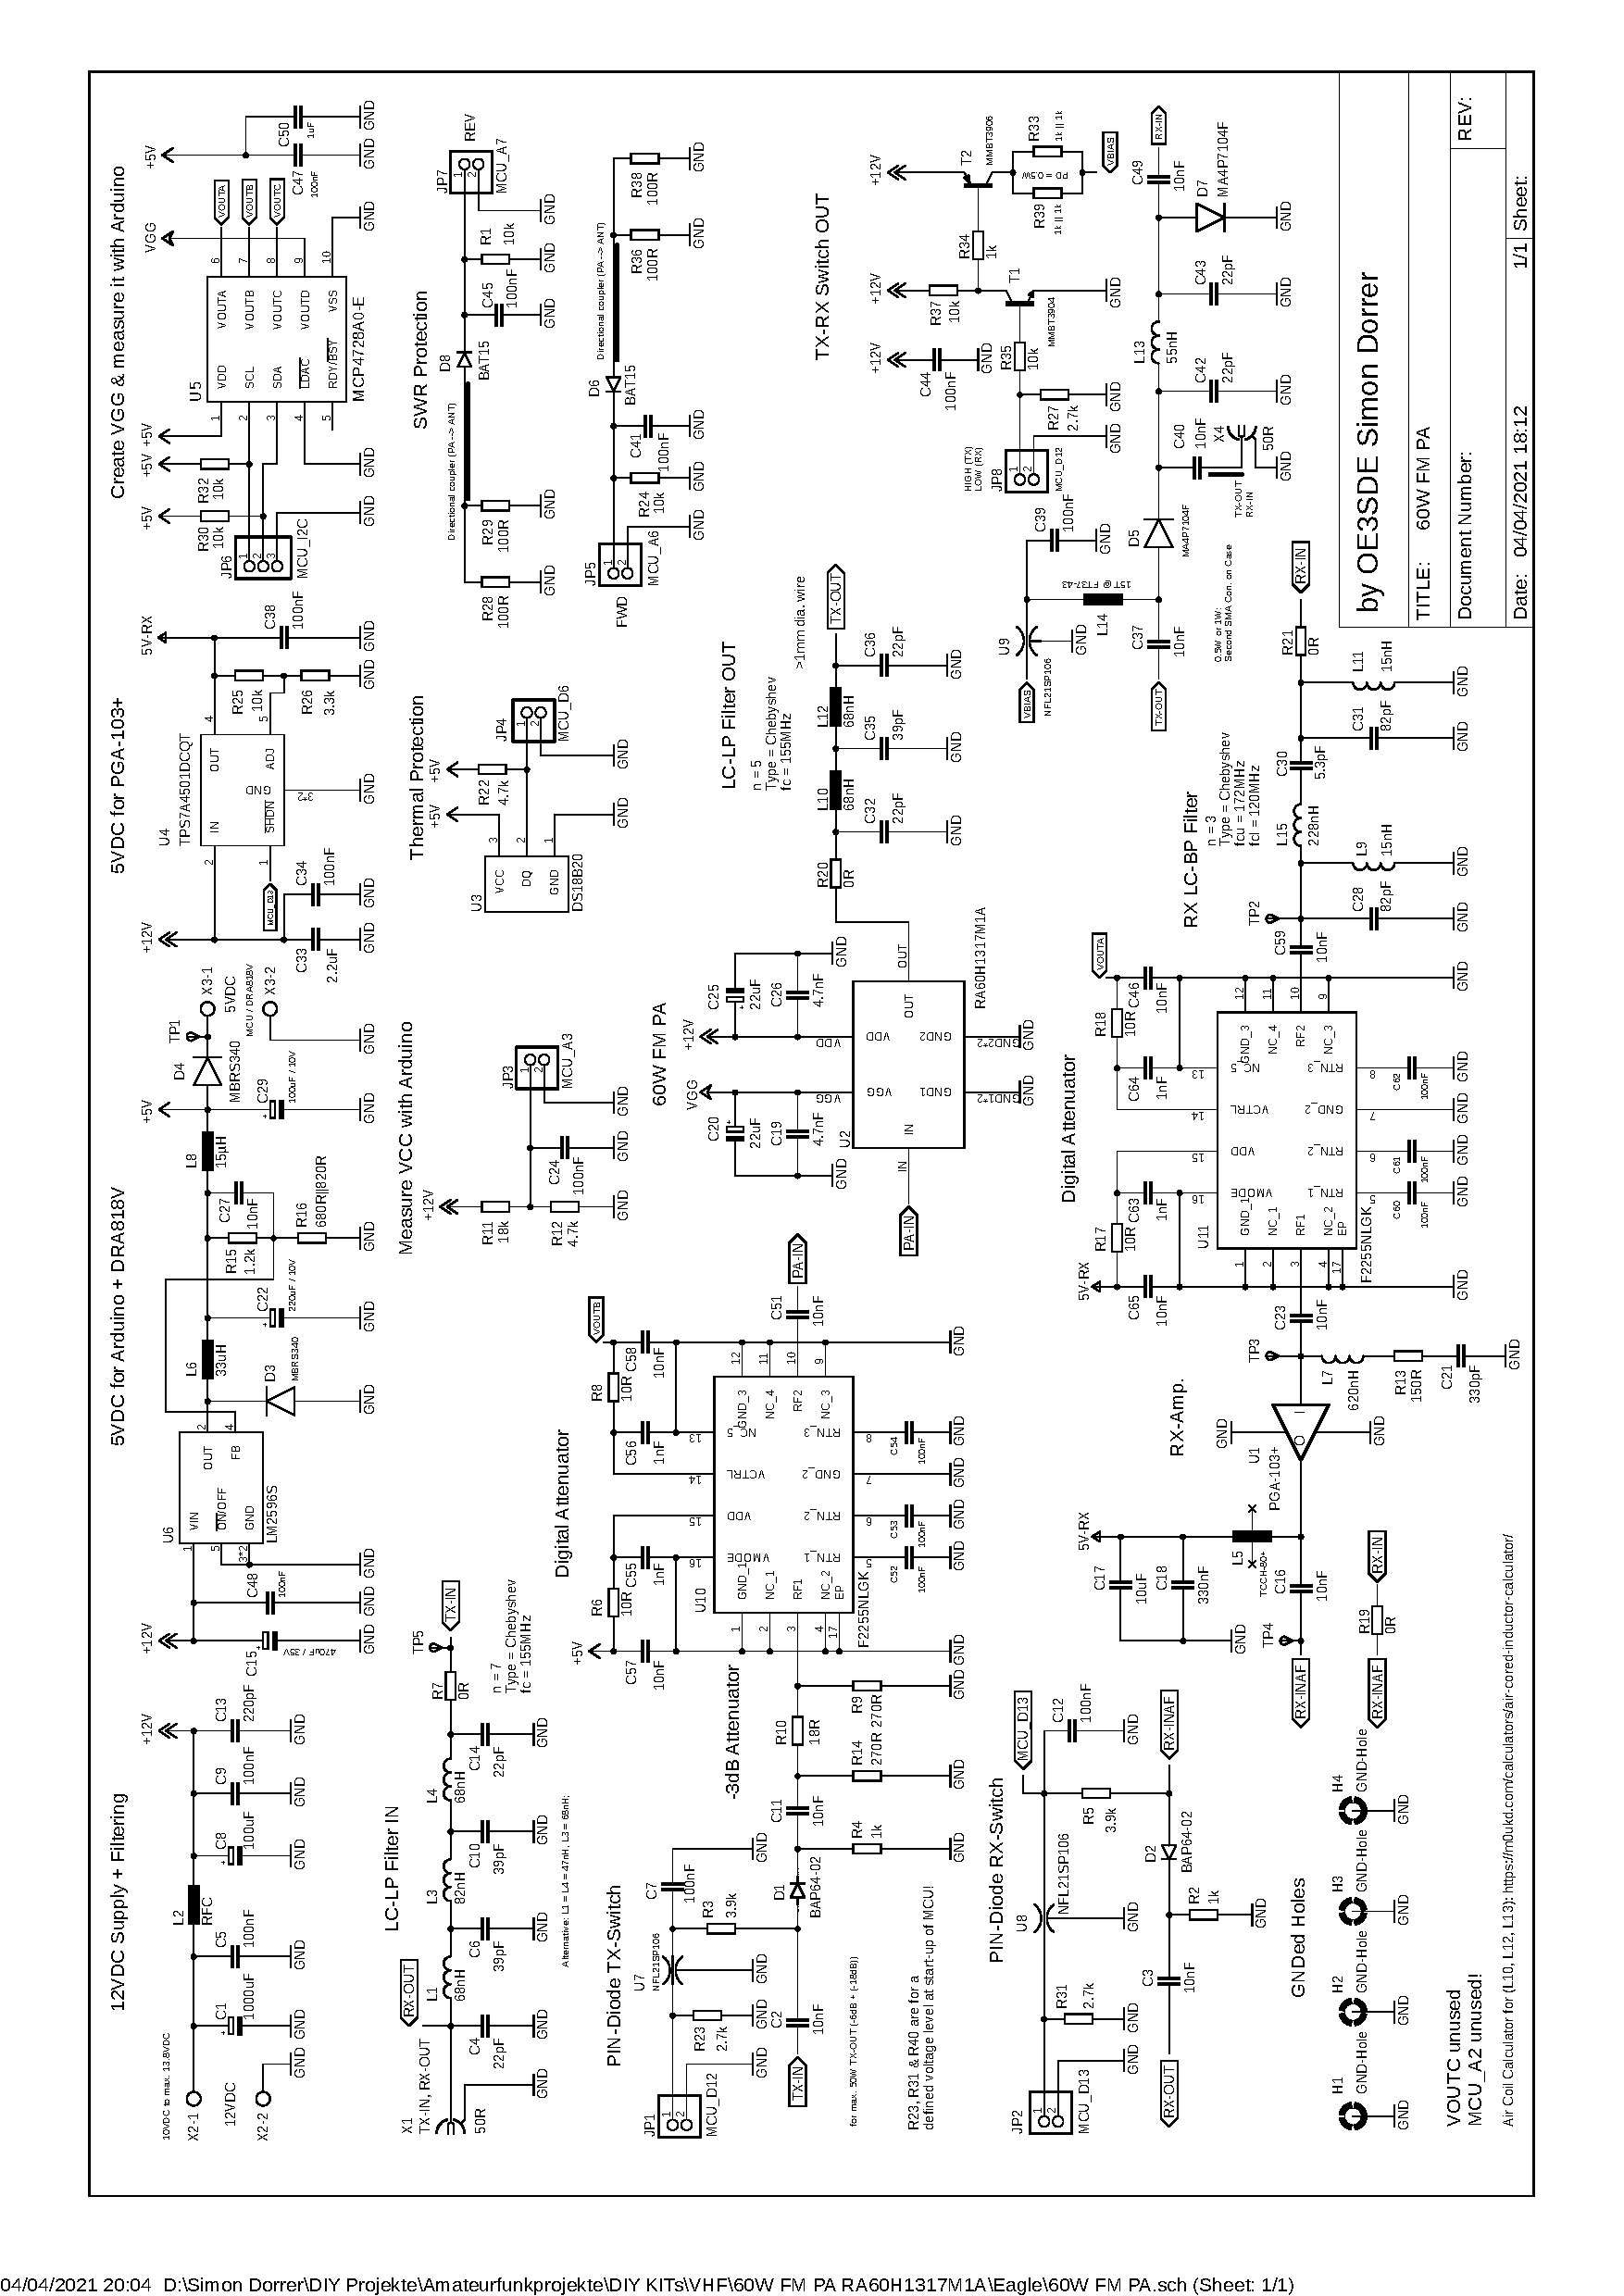
\includepdf[pages=-]{./2_circuit/60W FM PA_Circuit.pdf}
	
	% -- Chapter 3 ------------------------------------------------------------------------------------	
	\chapter{PCB}
	\label{chp:pcb}
	\section{Layer Stackup}
This \acs{PCB} is a two layer PCB. On the top layer the \acs{RF} signals and SMT components are placed. 
The bottom layer is a completed GND layer with some supply traces.
This PCB is produced by my sponsor JLCPCB \footnote{\url{https://jlcpcb.com/}}.
Normally, for bigger RF PCB-Designs a 4 layer PCB is used as follows: 

\begin{figure}[ht!]
	\centering
	\includegraphics[width = 15cm]{example-image}
	\caption{Two Layer PCB Stackup}
	\label{fig:PCB Layer Stackup}
\end{figure}
\newpage

\section{Coplanar Waveguide Grounded (CPWG)}
In RF PCB-Design applications it is very important, that the trace impedance is matched to 50$\Omega$.
Therefore, different techniques like Microstrip, Stripline or Coplanar Waveguide are used.
This PCB-Design uses the Coplanar Waveguide method. However, the calculation of this technique is not that easy (elliptical integrals etc.). That is why an online calculator \footnote{\url{https://chemandy.com/calculators/coplanar-waveguide-with-ground-calculator.htm}}  \cite{CPWGCalculator.2021} is used.
The original equations are in \cite{transmissionLineDesign} on page 79.

\subsection{RX CPWG Calculation}
	\begin{figure}[ht!]
		\centering
		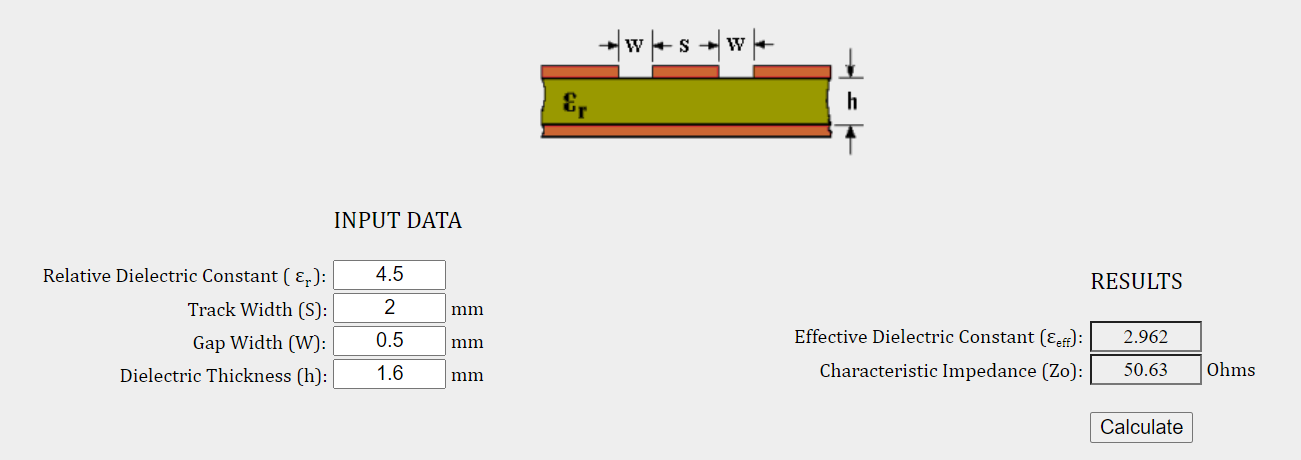
\includegraphics[width = 15cm]{./3_pcb/fig/CPWG_RX}
		\caption{RX CPWG Calculation}
		\label{fig:RX_CPWG}
	\end{figure}

\subsection{TX CPWG Calculation}
	\begin{figure}[ht!]
		\centering
		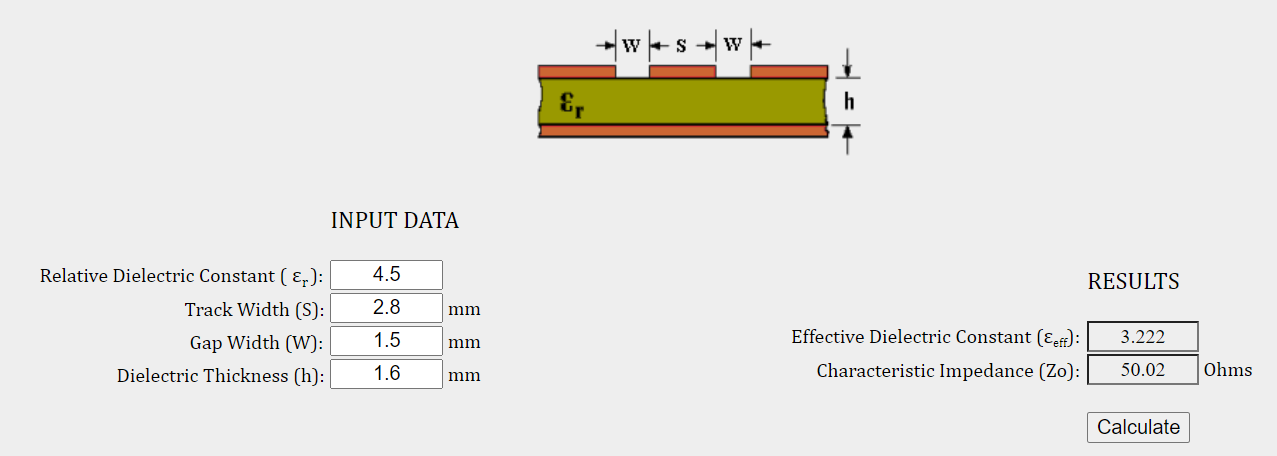
\includegraphics[width = 15cm]{./3_pcb/fig/CPWG_TX}
		\caption{TX CPWG Calculation}
		\label{fig:TX_CPWG}
	\end{figure}

\newpage
\section{Trace corners}	
	ToDo Text
	\begin{figure}[ht!]
		\centering
		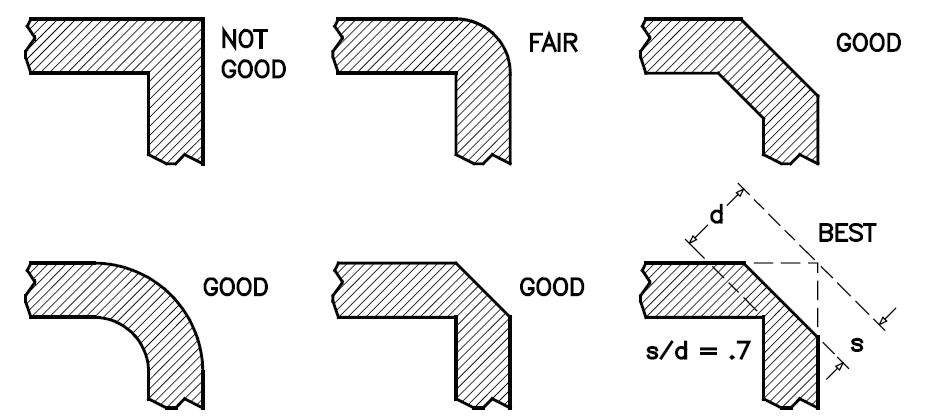
\includegraphics[width = 13cm]{./3_pcb/fig/Trace Corners}
		\caption{Corners in RF traces}
		\label{fig:Corners}
	\end{figure}

\section{3D PCB}	
	\begin{figure}[ht!]
		\centering
		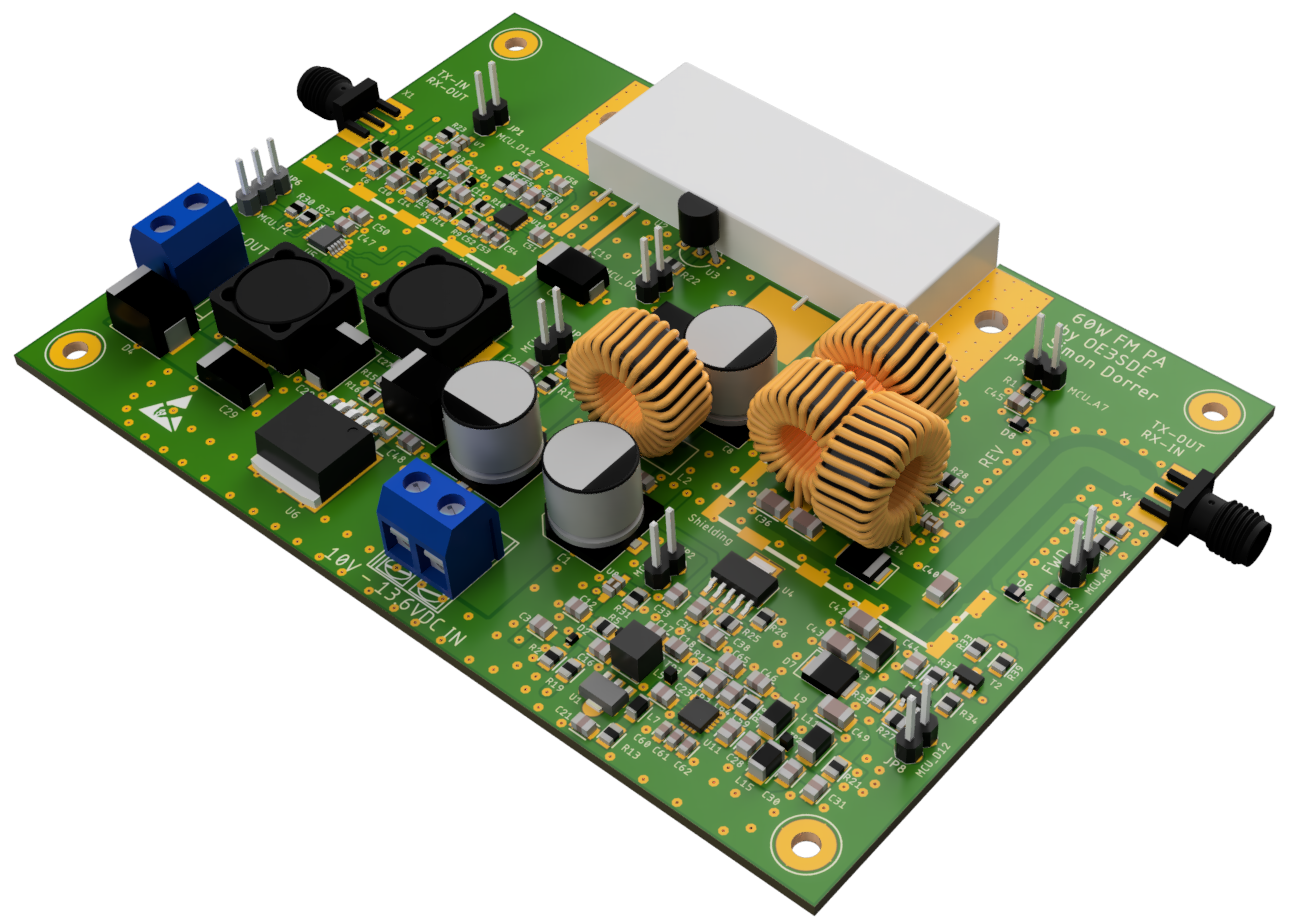
\includegraphics[width = 15cm]{./3_pcb/fig/3D-PCB}
		\caption{Finished \acs{PCB} 3D view}
		\label{fig:3D-PCB}
	\end{figure}

\newpage
\section{2D PCB}	
	\begin{figure}[ht!]
		\centering
		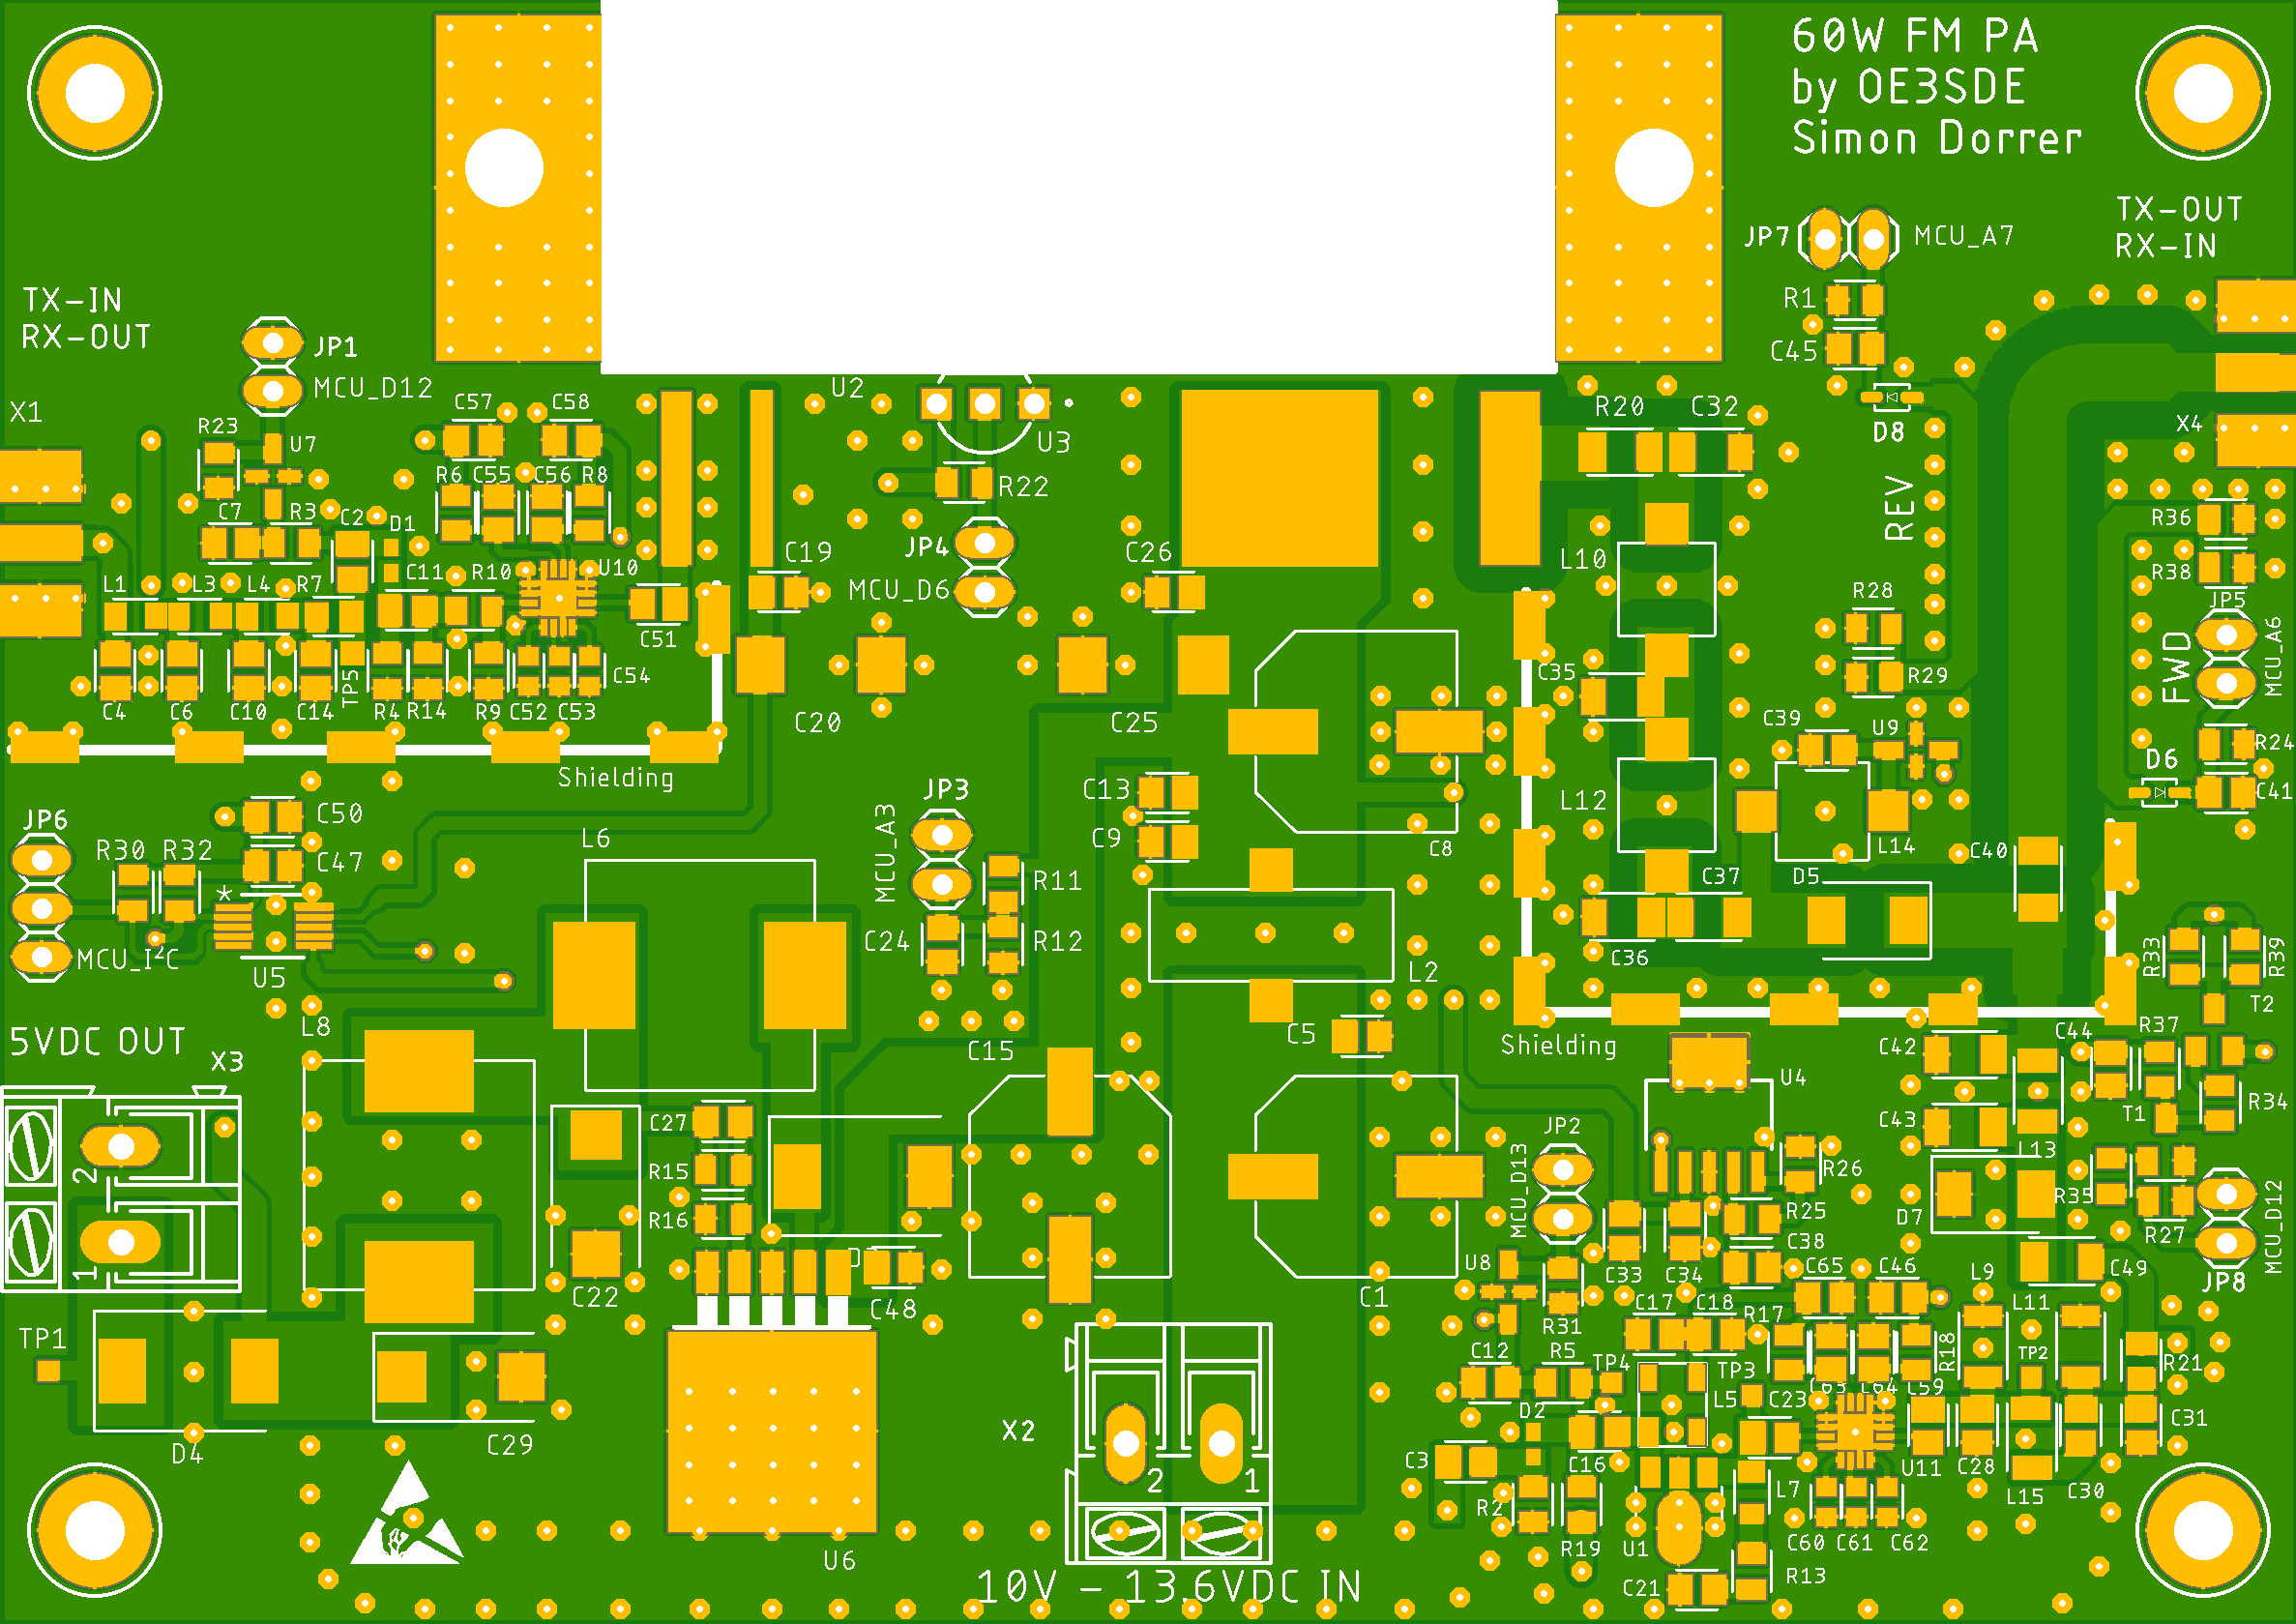
\includegraphics[width = 14cm]{./3_pcb/fig/PCB_Top}
		\caption{Finished \acs{PCB} 2D top view}
		\label{fig:PCB_Top}
	\end{figure}
	\bigskip
	\begin{figure}[ht!]
		\centering
		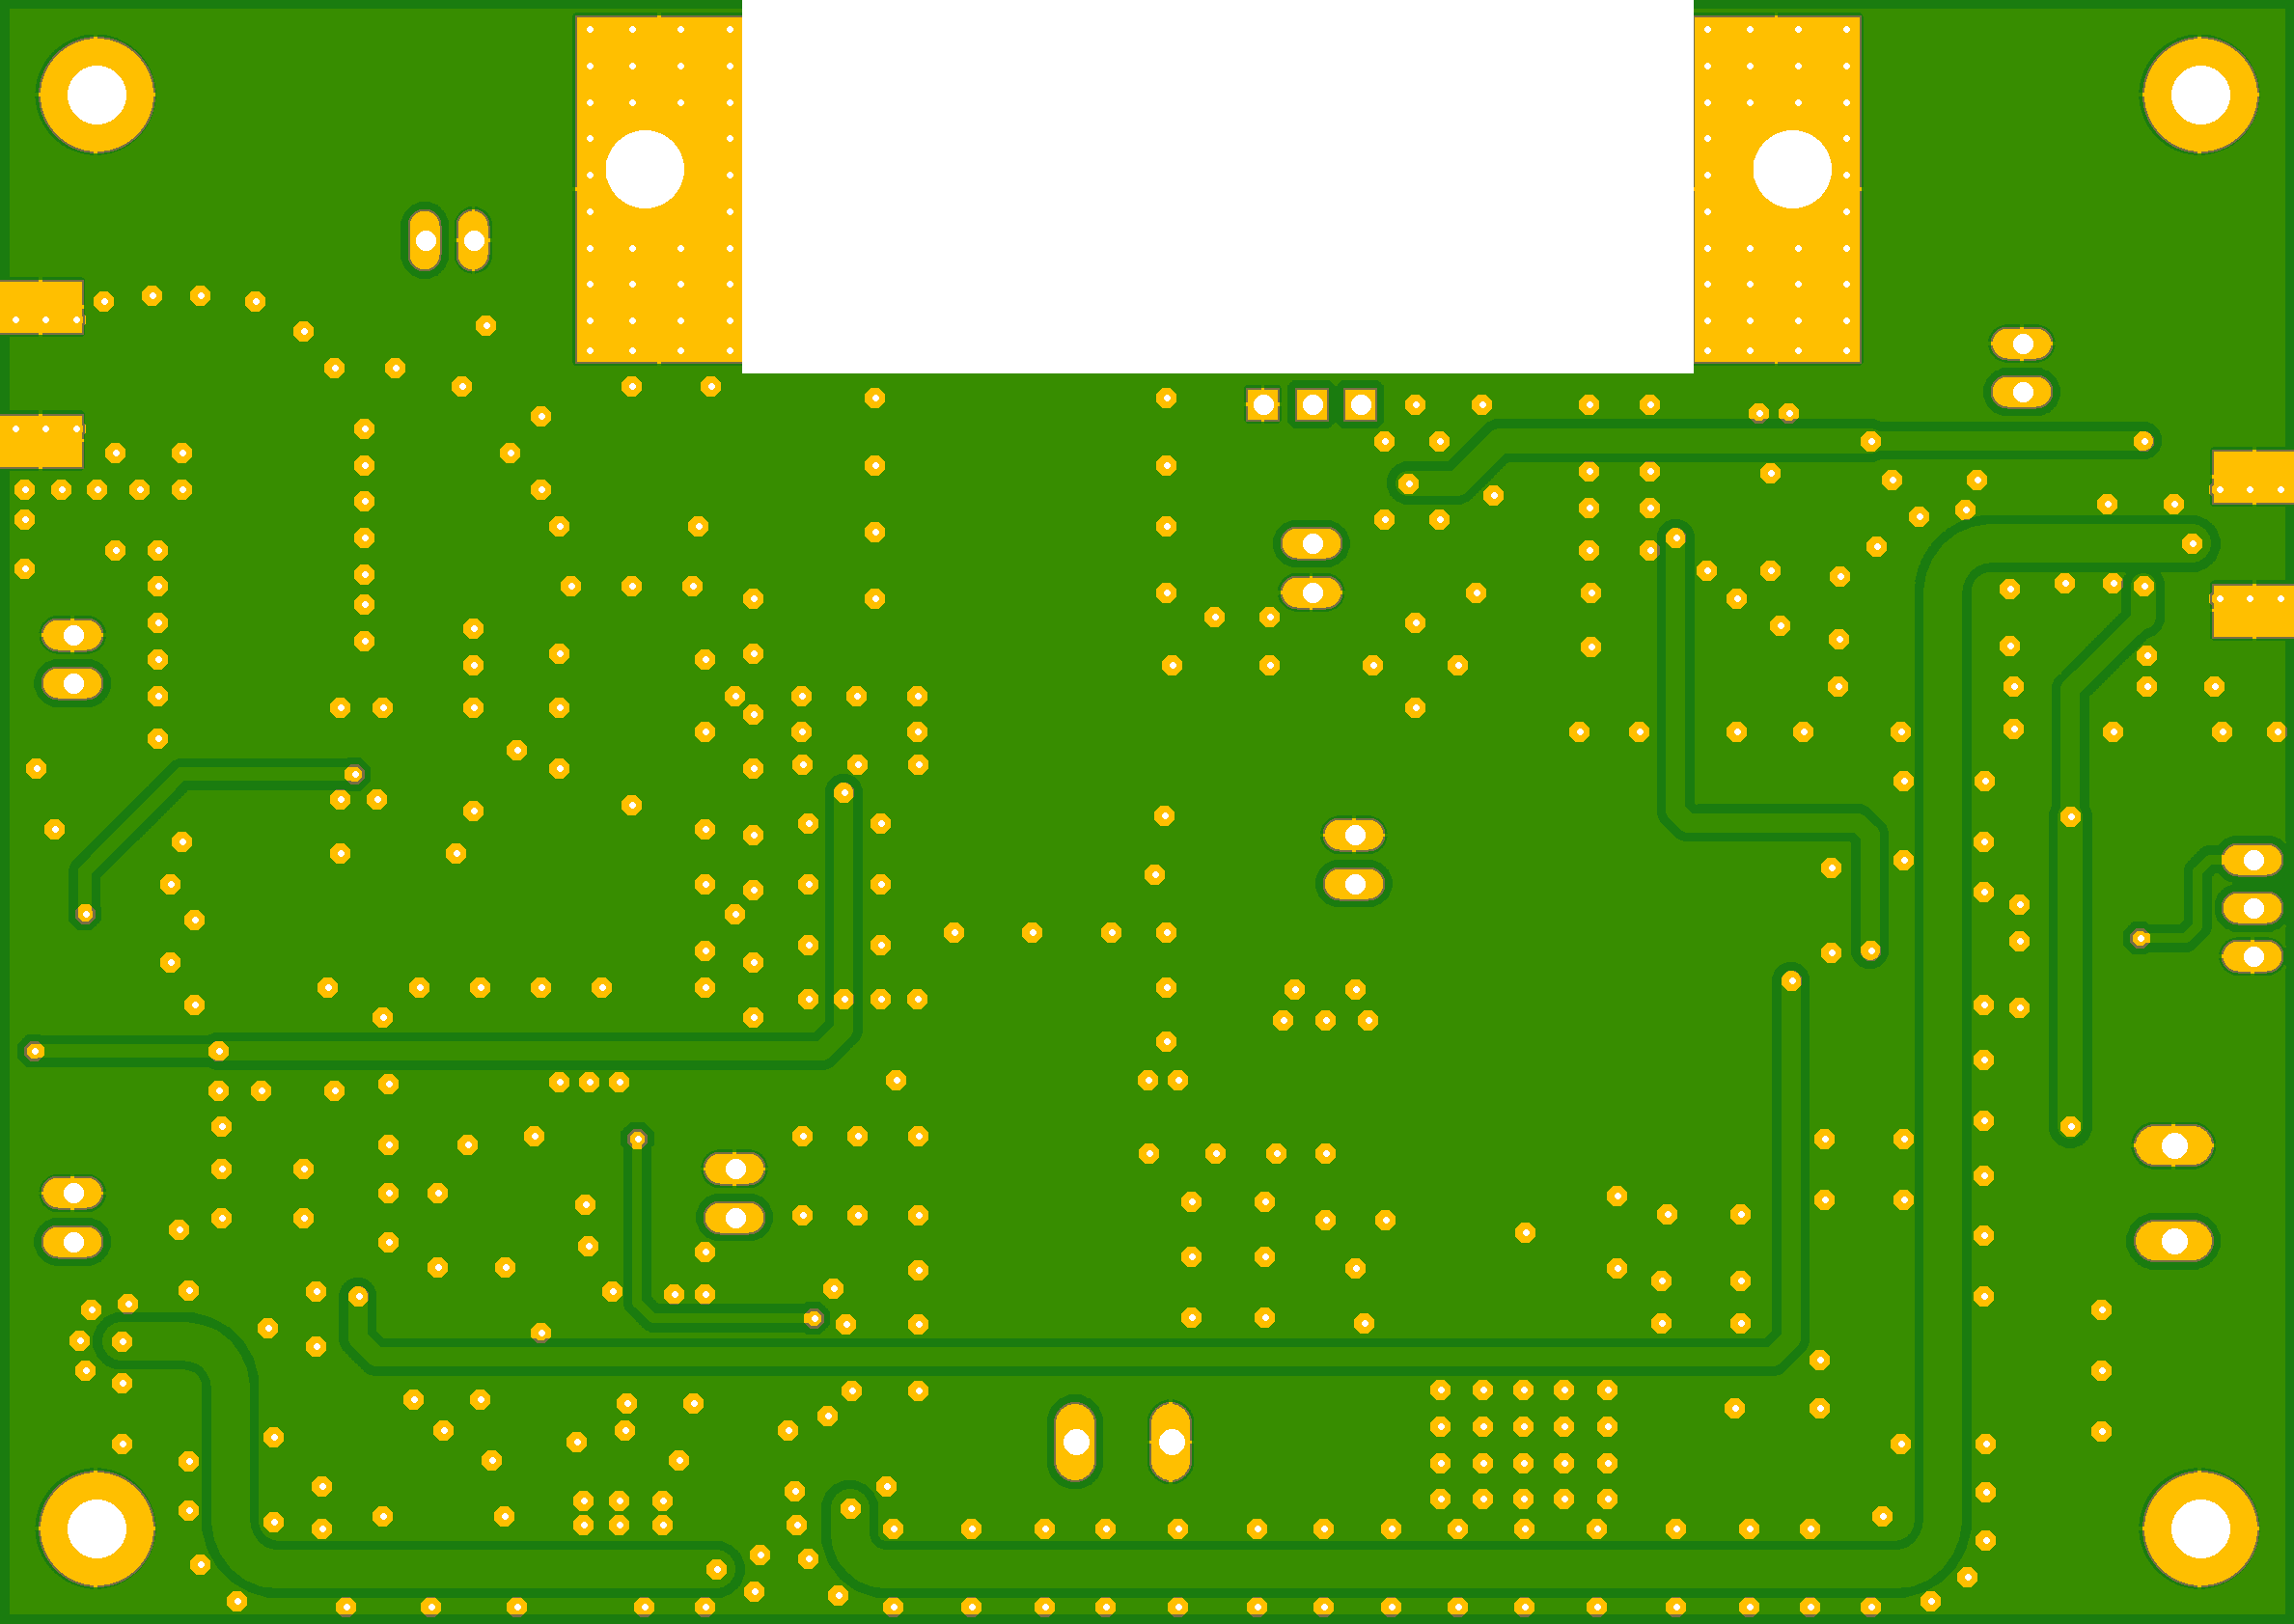
\includegraphics[width = 14cm]{./3_pcb/fig/PCB_Bot}
		\caption{Finished \acs{PCB} 2D bottom view}
		\label{fig:PCB_Bot}
	\end{figure}
\newpage
	
	% -- Chapter 4 ------------------------------------------------------------------------------------	
	\chapter{Bill of Material}
	\label{chp:bom}
	%Generated with https://www.tablesgenerator.com/latex_tables
\begin{longtable}{l|l|l}
	\label{long: BOM}
	Qty & Value         & Parts                                                        \\\hline
	
	\endhead
	
	4   & 0R            & R7, R19, R20, R21                                            \\
	1   & 1.2k          & R15                                                          \\
	1   & 1000uF        & C1                                                           \\
	4   & 100R          & R28, R29, R36, R38                                           \\
	6   & 100nF         & C52, C53, C54, C60, C61, C62                                 \\
	13  & 100nF         & C5, C7, C9, C12, C24, C34, C38, C39, C41, C44, C45, C47, C48 \\
	1   & 100uF         & C8                                                           \\
	1   & 100uF / 10V   & C29                                                          \\
	4   & 10R           & R6, R8, R17, R18                                             \\
	7   & 10k           & R1, R24, R25, R30, R32, R35, R37                             \\
	12  & 10nF          & C2, C3, C11, C16, C23, C27, C46, C51, C57, C58, C59, C65     \\
	3   & 10nF          & C37, C40, C49                                                \\
	1   & 10uF          & C17                                                          \\
	1   & 12VDC         & X2                                                           \\
	1   & 150R          & R13                                                          \\
	1   & 15T @ FT37-43 & L14                                                          \\
	2   & 15nH          & L9, L11                                                      \\
	1   & 15ÁH          & L8                                                           \\
	1   & 18R           & R10                                                          \\
	1   & 18k           & R11                                                          \\
	3   & 1k            & R2, R4, R34                                                  \\
	2   & 1k || 1k      & R33, R39                                                     \\
	4   & 1nF           & C55, C56, C63, C64                                           \\
	1   & 1uF           & C50                                                          \\
	1   & 2.2uF         & C33                                                          \\
	3   & 2.7k          & R23, R27, R31                                                \\
	1   & 220pF         & C13                                                          \\
	1   & 220uF / 10V   & C22                                                          \\
	1   & 228nH         & L15                                                          \\
	2   & 22pF          & C4, C14                                                      \\
	4   & 22pF          & C32, C36, C42, C43                                           \\
	2   & 22uF          & C20, C25                                                     \\
	2   & 270R          & R9, R14                                                      \\
	1   & 3.3k          & R26                                                          \\
	2   & 3.9k          & R3, R5                                                       \\
	1   & 330nF         & C18                                                          \\
	1   & 330pF         & C21                                                          \\
	1   & 33uH          & L6                                                           \\
	2   & 39pF          & C6, C10                                                      \\
	1   & 39pF          & C35                                                          \\
	2   & 4.7k          & R12, R22                                                     \\
	2   & 4.7nF         & C19, C26                                                     \\
	1   & 470uF / 35V   & C15                                                          \\
	1   & 5.3pF         & C30                                                          \\
	1   & 50R           & X4                                                           \\
	1   & 55nH          & L13                                                          \\
	1   & 5VDC          & X3                                                           \\
	1   & 620nH         & L7                                                           \\
	1   & 680R||820R    & R16                                                          \\
	2   & 68nH          & L10, L12                                                     \\
	2   & 68nH          & L1, L4                                                       \\
	1   & 82nH          & L3                                                           \\
	2   & 82pF          & C28, C31                                                     \\
	2   & BAP64-02      & D1, D2                                                       \\
	2   & BAT15         & D6, D8                                                       \\
	1   & DS18B20       & U3                                                           \\
	2   & F2255NLGK     & U10, U11                                                     \\
	4   & GND-Hole      & H1, H2, H3, H4                                               \\
	1   & LM2596S       & U6                                                           \\
	2   & MA4P7104F     & D5, D7                                                       \\
	2   & MBRS340       & D3, D4                                                       \\
	1   & MCP4728A0-E   & U5                                                           \\
	1   & MMBT3904      & T1                                                           \\
	1   & MMBT3906      & T2                                                           \\
	3   & NFL21SP106    & U7, U8, U9                                                   \\
	1   & PGA-103+      & U1                                                           \\
	1   & RA60H1317M1A  & U2                                                           \\
	1   & RFC           & L2                                                           \\
	1   & TCCH-80+      & L5                                                           \\
	1   & TPS7A4501DCQT & U4                                                           \\
	5   & TPSTP10SQ     & TP1, TP2, TP3, TP4, TP5                                      \\
	1   & TX-IN, RX-OUT & X1         												   \\
	
	\caption{Bill of Material}                                                 
\end{longtable}
	
	% -- Chapter 5 ------------------------------------------------------------------------------------	
	\chapter{Measurements}
	\label{chp:measurements}
	\section{TX-Path Transfer Function}
ToDo Text (Variable Gain with Vdd of RA60, XY V for every gain)

\subsection{TF of RA60H1317M1A}
	\begin{figure}[ht!]
		\centering
		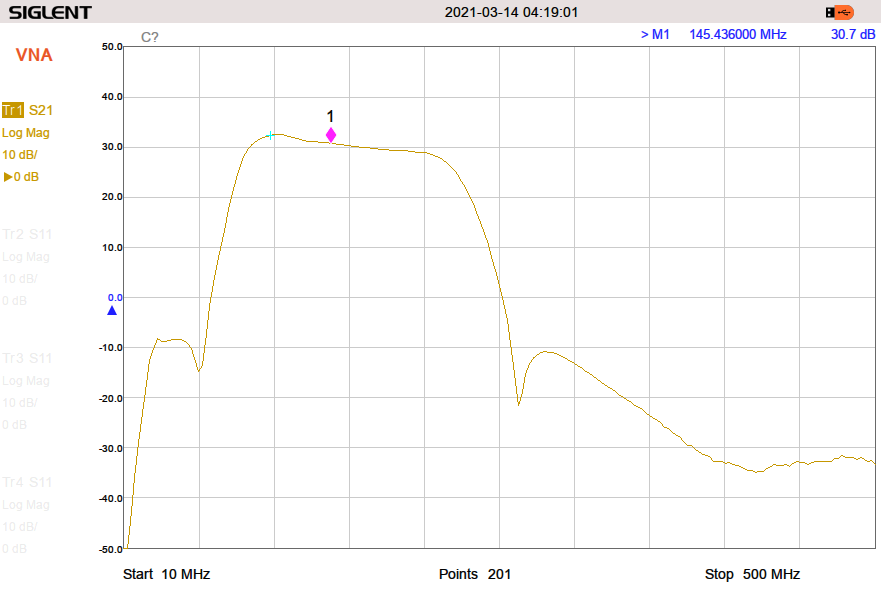
\includegraphics[width = 12cm]{./5_measurements/fig/RA60H-TF}
		\caption{Transfer Function of RA60H1317M1A}
		\label{fig:ra60h1317m1a TF}
	\end{figure}
	\newpage

\subsection{10dB Gain}
\begin{figure}[ht!]
	\centering
	\includegraphics[width = 12cm]{example-image}
	\caption{TX-Path Transfer Function with 10dB gain}
	\label{fig:10dB Gain}
\end{figure}

\subsection{30dB Gain}
	\begin{figure}[ht!]
		\centering
		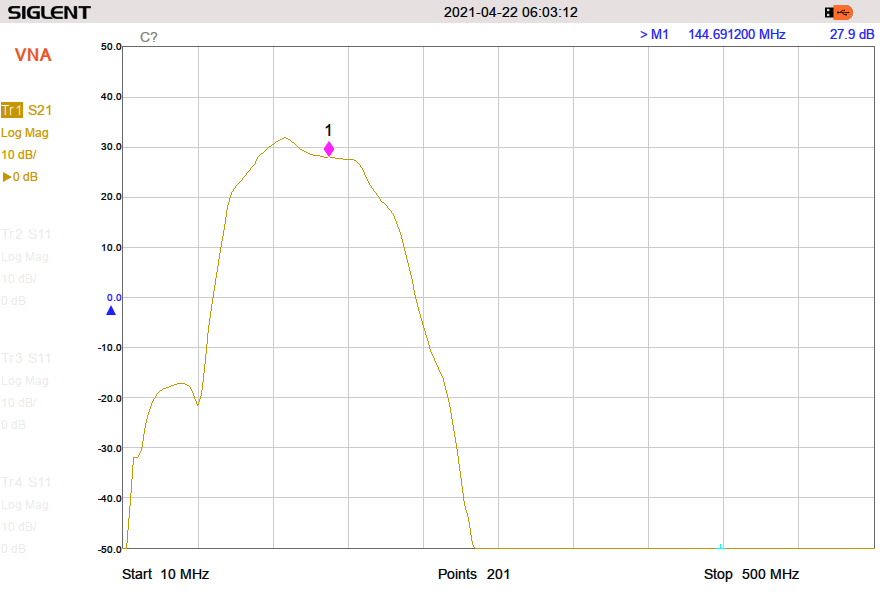
\includegraphics[width = 12cm]{./5_measurements/fig/TX-Path}
		\caption{TX-Path Transfer Function with 30dB gain}
		\label{fig:30dB Gain}
	\end{figure}
	\newpage
	
\section{RX-Path Transfer Function}
ToDo Text (Variable Attenuation with F2255)

\subsection{F2255NLGK Attenuation Diagram}
ToDo Text (What is a F2255)

	\begin{figure}[ht!]
		\centering
		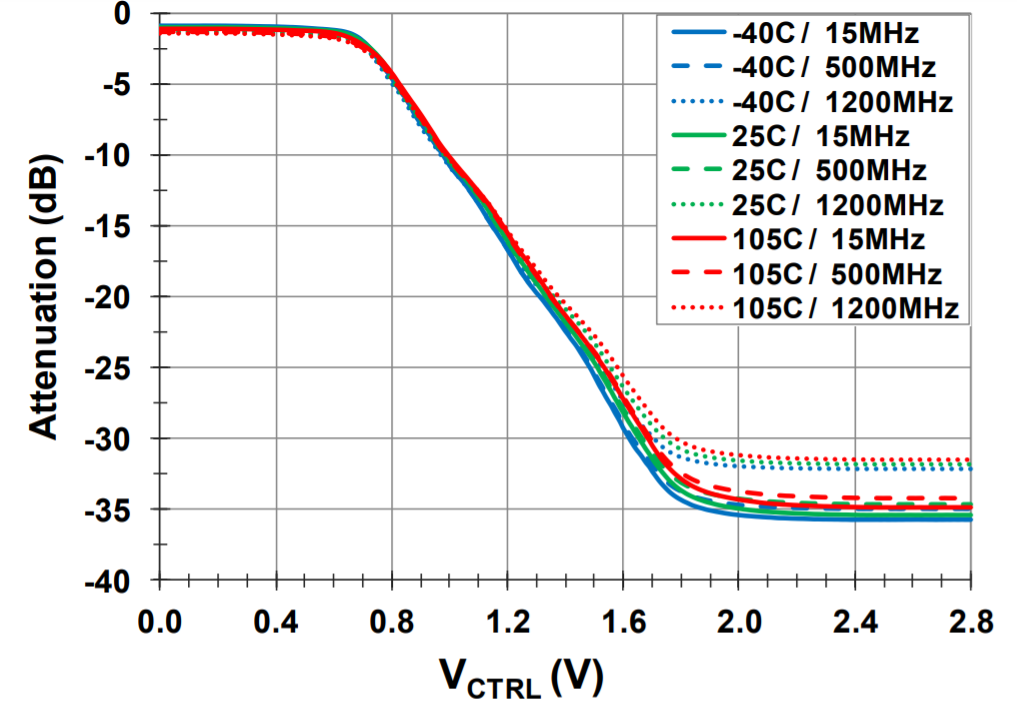
\includegraphics[width = 12cm]{./5_measurements/fig/F2255-Diagram}
		\caption{F2255NLGK Attenuation Diagram\protect\footnotemark \cite{f2255nlgk.2020}}
		\label{fig:F2255NLGK Att}
	\end{figure}

	\footnotetext{\url{https://www.mouser.at/datasheet/2/698/IDT_F2255_Datasheet_DST_20180209-1997542.pdf}}
	\newpage

\subsection{No Attenuation}
	\begin{figure}[ht!]
		\centering
		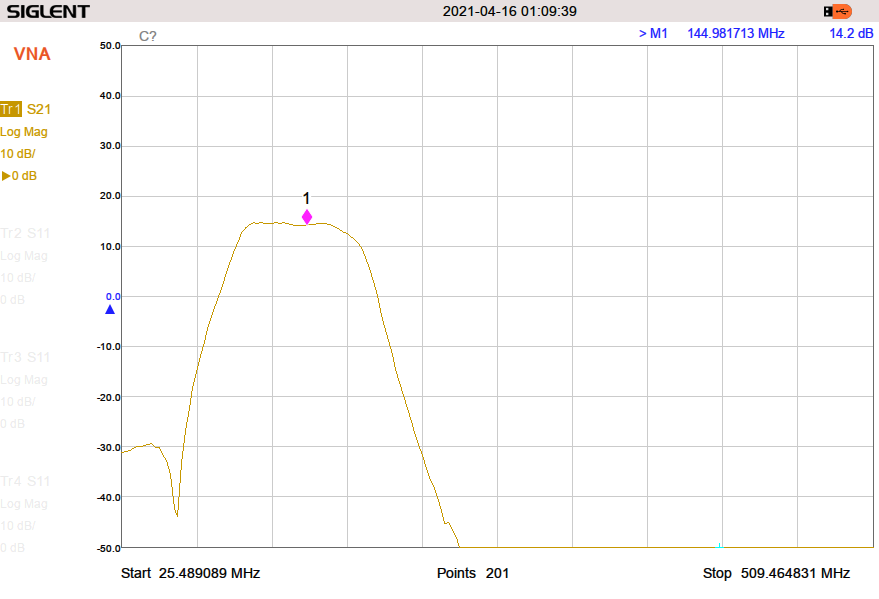
\includegraphics[width = 12cm]{./5_measurements/fig/RX-Path-NoAtt}
		\caption{RX-Path Transfer Function without attenuation}
		\label{fig:No Att}
	\end{figure}

\subsection{20dB Attenuation}
	\begin{figure}[ht!]
		\centering
		\includegraphics[width = 12cm]{example-image}
		\caption{RX-Path Transfer Function with 20dB attenuation}
		\label{fig:20dB Att}
	\end{figure}
	\newpage
	
\section{Output Power}
For all output power measurements an input power of XYdBm (xyW) is used.
Furthermore, at the input of the Vector Network Analyzer a 23dBm attenuator is mounted to handle the power.
So, the final output Power consists of the measured power and the 23dBm.\\
For exmaple, if the spectrum analyser shows an output power of XYdBm the output power equals $XY+23dBm = dBm (XYW)$.

\subsection{20W Output Power} 
	\begin{figure}[ht!]
		\centering
		\includegraphics[width = 12cm]{example-image}
		\caption{20W Output Power}
		\label{fig:20W OUT}
	\end{figure}
	\newpage

\subsection{40W Output Power}
	\begin{figure}[ht!]
		\centering
		\includegraphics[width = 12cm]{example-image}
		\caption{40W Output Power}
		\label{fig:40W OUT}
	\end{figure}

\subsection{60W Output Power}
	\begin{figure}[ht!]
		\centering
		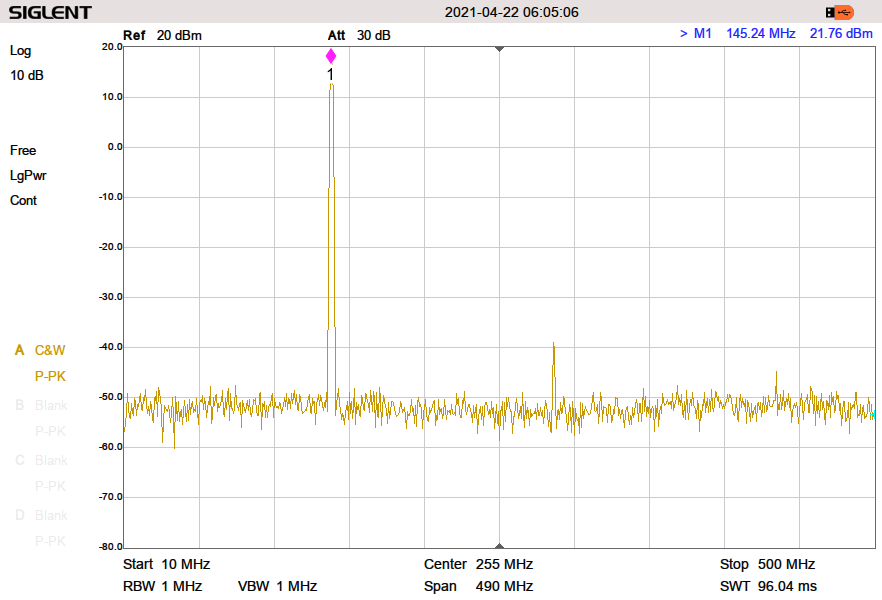
\includegraphics[width = 12cm]{./5_measurements/fig/60W-Out}
		\caption{60W Output Power}
		\label{fig:60W OUT}
	\end{figure}
	
	% -- Chapter 6 ------------------------------------------------------------------------------------	
	\chapter{Microcontroller Code}
	\label{chp:code}
	In this chapter, the MCU Code written with Arduino IDE is implemented. 
The internal hardware of the used MCU (ATmega328) is programmed on register level.
To control the OLED display, the external DAC and some sensors, external libraries are used.

\begin{lstlisting}[language=Arduino]
//Arduino Code for DRA818V FM TRX + 60W RA60H1317M1A
//This code is written by OE3SDE, Simon Dorrer!

//Define CPU-Clock-Speed (16MHz internal clock)
//#define F_CPU 16000000UL

//Define Baudrate for UART
//#define BAUD 9600UL

//Include Libraries
#include <avr/io.h>
#include <stdio.h>
#include <avr/interrupt.h>

//I2C
#include <Wire.h>

//MCP4728
#include <Adafruit_MCP4728.h>

//DS18B20
#include <OneWire.h> 
#include <DallasTemperature.h>

//Libs. for SD1306 OLED-Display
#include <Adafruit_GFX.h>               // Include core graphics library for the display
#include <Adafruit_SSD1306.h>           // Include Adafruit_SSD1306 library to drive the display
#include <Fonts/FreeMono9pt7b.h>        // Add a custom font
/*List of different fonts :
FreeMono9pt7b.h
FreeMonoBold9pt7b.h
FreeMonoBoldOblique9pt7b.h
FreeMonoOblique9pt7b.h  
*/
//----------------------------------------------------------------------------

//Definitions
//I/O Declaration
//1W FM TRX Board (DRA818V)
//#define TX        0     //PD0 / D0
//#define RX        1     //PD1 / D1
#define SW1         2     //PD2 / D2 - INT0
#define PTT_IN      3     //PD3 / D3 - INT1
#define PTT_OUT     7     //PD7 / D7
#define PD          0     //PB0 / D8
#define H_L         1     //PB1 / D9
#define HC05_TX     2     //PB2 / D10
#define HC05_RX     3     //PB3 / D11
#define E1          0     //PC0 / A0
#define E2          1     //PC1 / A1

//60W FM TRX Board (RA60H1317M1A)
#define PGA_SHDN    5     //PB5 / D13 (LOW --> PGA OFF, HIGH --> PGA ON) + RX Switch
#define TX_SW       4     //PB4 / D12 (HIGH TX Switch)
//#define T1_SW     7     //PD7 / D7  (switches T1 for TRX Switch - LOW for TX, HIGH for RX) --> see PTT_OUT D7
#define DS18B20_OW  6     //PD6 / D6  (One wire input of DS18B20 Temp. Sensor)
#define SWR_REV     7     //PC7 / A7  (ADC samples reverse voltage)
#define SWR_FWD     6     //PC6 / A6  (ADC samples forward voltage)
#define ADC_VDD     3     //PC3 / A3  (ADC samples VDD voltage) 

//I2C: OLED Display, MCP4728

//Makros
//RX or TX ATTENUATOR
#define RX_ATTENUATOR_CHANNEL  MCP4728_CHANNEL_A
#define TX_ATTENUATOR_CHANNEL  MCP4728_CHANNEL_B

//PA max. ratings
#define VDD_LOWER_LIMIT 10.7  //in V
#define VDD_UPPER_LIMIT 14.2  //in V
#define SWR_LOWER_LIMIT 0.5   
#define SWR_UPPER_LIMIT 2
#define HEAT_UPPER_LIMIT 45   //in degrees
//----------------------------------------------------------------------------

//Global variables / Objects
uint8_t TX = 0;  // 0... RX; 1... TX
uint8_t switched = 0;

//OLED
Adafruit_SSD1306 display(128, 64);    // Create display
volatile uint16_t timer1Count = 0;

//DRA818 Variables
typedef struct{
	float txFreq;         //TX-Frequency in MHz (134.0000 - 174.0000)
	float rxFreq;         //RX-Frequency in MHz (134.0000 - 174.0000)
	String txCTCSS;       //CTCSS frequency (0000 - 0038); 0000 = "no CTCSS" 
	String rxCTCSS;       //CTCSS frequency (0000 - 0038); 0000 = "no CTCSS" 
	uint8_t bw;           //Bandwith in KHz (0= 12.5KHz or 1= 25KHz)
	uint8_t squ;          //Squelch level  (0 - 8); 0 = "open" 
	uint8_t vol;
	uint8_t prf;
	uint8_t hpf;
	uint8_t lpf;
}DRA818;

DRA818 dra818 = {145.5000, 145.5000, "0000", "0000", 1, 4, 8, 0, 0, 0};

//DS18B20
OneWire oneWire(DS18B20_OW); 
DallasTemperature ds18b20(&oneWire);

//MCP4728
Adafruit_MCP4728 mcp4728;

//Rotary Encoder Variables
int counter = 0; 
int aState;
int aLastState;  

//RA60H1317M1A Variables
float txGain = 10;
float txAtt = 0;
float rxAtt = 0;
uint8_t monitorPA = 0;  //monitorPA = 1... PA is OK!
//----------------------------------------------------------------------------

//Subprograms
//Hardware Init Methods
void IO_Init()                  //initialize IO
{
	//Define INPUTs
	DDRD &= ~(1 << SW1);          //set PD2 (SW1) as Input
	PORTD |= (1 << SW1);          //activate Pull-Up-R at PD2 (SW1)    
	
	DDRD &= ~(1 << PTT_IN);       //set PD3 (PTT-IN) as Input
	PORTD |= (1 << PTT_IN);       //activate Pull-Up-R at PD3 (PTT_IN)     
	
	DDRC &= ~(1 << E1);           //set PC0 (E1) as Input    
	DDRC &= ~(1 << E2);           //set PC1 (E2) as Input
	
	DDRC &= ~(1 << ADC_VDD);      //set PC3 (ADC_VDD) as Input  
	//PORTC |= (1 << ADC_VDD);      //activate Pull-Up-R at PC3 (ADC_VDD)
	
	DDRC &= ~(1 << SWR_FWD);      //set PC6 (SWR_FWD) as Input  
	PORTC |= (1 << SWR_FWD);      //activate Pull-Up-R at PC6 (SWR_FWD)
	
	DDRC &= ~(1 << SWR_REV);      //set PC7 (SWR_REV) as Input  
	PORTC |= (1 << SWR_REV);      //activate Pull-Up-R at PC7 (SWR_REV)
	
	//Define OUTPUTs
	DDRD |= (1 << PTT_OUT);       //set PD7 (PTT_OUT) as Output
	DDRB |= (1 << PD);            //set PB0 (PD) as Output
	DDRB |= (1 << H_L);           //set PB1 (H_L) as Output
	
	DDRB |= (1 << TX_SW);         //set PB4 (TX_Switch) as Output
	DDRB |= (1 << PGA_SHDN);      //set PB5 (PGA_SHDN) as Output
}

void Timer1_COMPA_Init()
{
	//Control Registers
	TCCR1A = 0; TCCR1B = 0; TCCR1C = 0; //Reset
	
	// set CTC mode
	//TCCR1A |= (1 << WGM10);
	//TCCR1A |= (1 << WGM11);
	TCCR1B |= (1 << WGM12);
	
	// Set Prescaler 1024 (TCCR1B = (1 << WGM12) | (0x5 << CS10);)
	TCCR1B |= (1 << CS12);
	TCCR1B &= ~(1 << CS11);
	TCCR1B |= (1 << CS10);
	
	// initialize compare value
	OCR1A = 16;
	
	// enable timer compare interrupt
	TIMSK1 |= (1 << OCIE1A);
}

void Timer2_COMPA_Init()
{
	//Timer2 settings
	TCCR2A = 0x00; TCCR2B = 0x00; //Reset
	
	//Enable Timer2 CTC Mode
	//TCCR2A |= (1 << WGM20);
	TCCR2A |= (1 << WGM21);
	//TCCR2B |= (1 << WGM22);
	
	//Prescaler
	// 1024 prescaling for Timer2 (TCCR2B = (0x7 << CS20);)
	TCCR2B |= (1 << CS20);
	TCCR2B |= (1 << CS21);
	TCCR2B |= (1 << CS22);
	
	//Initialize compare value
	OCR2A = 0;
	
	//initialize TIMER0-Counter
	//TCNT2 = 0; // set counter value FORMEL: x = maximaler Zaehlwert - ((CPUtakt/PRESCALER)/ gesuchte Frequenz)
	
	//disable Timer compare interrupt
	TIMSK2 &= ~(1 << OCIE2A);
}

void INT0_Init()
{
	//enable Interrupt
	EIMSK |= (1 << INT0); //Ext. Int0 ein
	
	//Set falling Edge Interrupt (EICRA |= (0x2 << ISC00);)
	EICRA &= ~(1 << ISC00);
	EICRA |= (1 << ISC01);
}
void INT1_Init()
{
	//enable Interrupt
	EIMSK |= (1 << INT1); //Ext. Int1 ein
	
	//Set rising & falling Edge Interrupt (EICRA |= (0x2 << ISC10);)
	EICRA |= (1 << ISC10);
	EICRA &= ~(1 << ISC11);
}

void ADC_Init()
{
	//ADC Setup
	//Set Reference Voltage (VCC = VREF)
	ADMUX &= ~(1 << REFS1);
	ADMUX |= (1 << REFS0);
	
	//Prescaler --> 128 (50kHz - 200kHz)
	ADCSRA |= (1 << ADPS0);
	ADCSRA |= (1 << ADPS1);
	ADCSRA |= (1 << ADPS2);
	
	ADCSRA |= (1 << ADEN); //Enable ADC
	
	//Dummy Readout to warm up the ADC
	ADCSRA |= (1<<ADSC);          //Start ADC conclusion
	while (ADCSRA & (1<<ADSC)){}  //wait until ADC is ready
	(void) ADC;
}
uint16_t ADC_ReadValue(uint8_t channel)
{
	ADMUX = (ADMUX & ~(0x1F)) | (channel & 0x1F); //which ADCx? Bit Mask to secure ADMUX settings in Init() function
	
	ADCSRA |= (1<<ADSC);          //Start ADC conclusion
	while (ADCSRA & (1<<ADSC)){}  //wait until ADC is ready
	
	return ADC;                   //return the ADC value
}

//DRA818V Methods
void DRA818V_setGroup()
{
	Serial.print("AT+DMOSETGROUP=");         // begin message
	Serial.print(dra818.bw);
	Serial.print(",");
	Serial.print(dra818.txFreq, 4);
	Serial.print(",");
	Serial.print(dra818.rxFreq, 4);
	Serial.print(",");
	Serial.print(dra818.txCTCSS);
	Serial.print(",");
	Serial.print(dra818.squ);
	Serial.print(",");
	Serial.println(dra818.rxCTCSS);
}
void DRA818V_setVolume()
{
	Serial.print("AT+DMOSETVOLUME=");
	Serial.println(dra818.vol);
}
void DRA818V_setFilter()
{
	Serial.print("AT+SETFILTER=");
	Serial.print(dra818.prf);
	Serial.print(",");
	Serial.print(dra818.hpf);
	Serial.print(",");
	Serial.println(dra818.lpf);
}
void DRA818V_Init()             // initialize DRA818V
{
	PORTB &= ~(1 << PD);
	delay(2000);
	
	//I/O
	PORTD |= (1 << PTT_OUT);      // set PD7 (PTT_OUT) HIGH at the beginning (RX-Mode)
	PORTB |= (1 << PD);           // set PB0 (PD) HIGH at the beginning (Normal-Mode)
	PORTB &= ~(1 << H_L);         // set PB1 (H/L) LOW at the beginning (LOW-Power = 0.5W)
	
	//UART
	Serial.begin(9600);
	delay(10);
	DRA818V_setGroup();
	delay(500);
	DRA818V_setVolume();
	delay(500);
	DRA818V_setFilter();
	delay(500);
}

//RA60H1317M1A Methods
float getVDD()      //Get VDD Voltage (10.8VDC to 13.6VDC)
{
	float vdd = 0;
	// #PJN: You may spend a LOT of time in this loop => make ADC reading asynchronous
	
	vdd = ADC_ReadValue(ADC_VDD) * 5.0 / 1024.0;
	
	return((vdd * ((4700 + 18000) / 4700)) + 2.2);  //returns supply voltage without voltage division (magic numbers equals the voltage divider resistor values)
}
float getSWR()      //Get SWR of output load (should be between 0.5 and 2)
{
	float rev = 0;
	float fwd = 0;
	// #PJN: You may spend just more time in this loop => make ADC reading asynchronous
	for(int i = 0; i < 10; i++)   //10 iterations for a more precise result
	{
		rev = rev + ADC_ReadValue(SWR_REV);
		fwd = fwd + ADC_ReadValue(SWR_FWD);
	}
	rev = rev / 10 / 1024 * 5;
	fwd = fwd / 10 / 1024 * 5;
	
	//SWR Calculation
	return((fwd + rev) / (fwd - rev));
}
float getPWR()
{
	float fwd = 0;
	for(int i = 0; i < 10; i++)   //10 iterations for a more precise result
	{
		fwd = fwd + ADC_ReadValue(SWR_FWD);
	}
	fwd = fwd / 10 / 1024 * 5;
	
	//PWR Calculation
	return((fwd * fwd) / 50);
}
float getHeat()     //Get heat of RA60H1317M1A measured by DS18B20, should be smaller than 50
{
	ds18b20.requestTemperatures();
	return(ds18b20.getTempCByIndex(0));
}
void setTXGain(float gain)  //Set Gain of RA60H1317M1A via MCP4728 (VOUTD)
{
	if(gain == 0)
	{
		mcp4728.setChannelValue(MCP4728_CHANNEL_D, 0);
	}
	else
	{
		//ToDo Formula
		mcp4728.setChannelValue(MCP4728_CHANNEL_D, 4095);
	}
}
void setAttenuation(MCP4728_channel_t channel, float att) //Attenuation of U11 (RX) or U12 (TX) (F2255NLGK)
{
	//Note that the PGA-103 has a constant gain of 25dB for RX path! RX_ATTENUATOR_CHANNEL MCP4728_CHANNEL_A
	//Note that an 6dB Attenuator is assembled on board for TX path! TX_ATTENUATOR_CHANNEL MCP4728_CHANNEL_B
	
	if(att > 35)
	{
		mcp4728.setChannelValue(channel, 2048);
	}
	else if(att < 2.5)
	{
		mcp4728.setChannelValue(channel, 0);
	}
	else
	{
		att = att * (-1);
		mcp4728.setChannelValue(channel, (uint16_t)(4096 * (-0.03692 * att + 0.60769) / 5));  //0.7V (-2.5dB) to 1.9V (-35dB), magic numbers are calculated according to the attenuation curve of the datasheet!
	}
}
void switchPAtoTX(uint8_t TX_Att, uint8_t TX_Gain)
{
	if(monitorPA == 1)
	{
		//turn OFF RX:
		mcp4728.setChannelValue(MCP4728_CHANNEL_C, 0);    //turn RX Path in TRX Switch OFF (VOUTC to LOW)
		PORTB &= ~(1 << PGA_SHDN);                        //turn OFF PGA RX-Amp. and RX Switch (D13 to LOW)
		setAttenuation(RX_ATTENUATOR_CHANNEL, 36);        //set full attenuation of U11 (F2255NLGK)
		
		delay(100);     //100ms settling time
		
		//turn ON TX:
		PORTD &= ~(1 << PTT_OUT);                         //turn TX Path in TRX Switch ON (D7 LOW)
		PORTB |= (1 << TX_SW);                            //turn on TX Switch (D12 to HIGH)
		setAttenuation(TX_ATTENUATOR_CHANNEL, TX_Att);    //set attenuation of U12 (F2255NLGK)
		setTXGain(TX_Gain);                               //Set TX gain (VGG (Gate) voltage) of RA60H1317M1A
		delay(100);                                       //100ms settling time
	}
	else
	{
		switchPAtoRX(rxAtt);
	}
}
void switchPAtoRX(float RX_Att)
{
	//turn OFF TX:
	setTXGain(0);                                       //Set gain of RA60H1317M1A to 0
	setAttenuation(TX_ATTENUATOR_CHANNEL, 36);          //set full attenuation of U12 (F2255NLGK)
	PORTB &= ~(1 << TX_SW);                             //turn OFF TX Switch (D12 to LOW)
	PORTD |= (1 << PTT_OUT);                            //turn TX Path in TRX Switch OFF (D7 HIGH)
	delay(100);                                         //100ms settling time
	
	//turn ON RX
	mcp4728.setChannelValue(MCP4728_CHANNEL_C, 4095);   //turn RX Path in TRX Switch ON (VOUTC to HIGH)
	PORTB |= (1 << PGA_SHDN);                           //turn ON PGA RX-Amp. and RX Switch (D13 to HIGH)
	setAttenuation(RX_ATTENUATOR_CHANNEL, RX_Att);      //set attenuation of U11 (F2255NLGK)
	delay(100);                                         //100ms settling time
}
void verifyPA()   //Shutdown RA60H1317M1A according to SWR, VDD and Heat
{
	float vdd = getVDD();
	float swr = getSWR();
	float heat = getHeat();
	Serial.print("VDD: ");
	Serial.println(vdd);
	Serial.print("SWR: ");
	Serial.println(swr);
	Serial.print("HEAT: ");
	Serial.println(heat);
	
	//if((vdd >= VDD_LOWER_LIMIT && vdd <= VDD_UPPER_LIMIT) && (swr >= SWR_LOWER_LIMIT && swr <= SWR_UPPER_LIMIT) && heat <= HEAT_UPPER_LIMIT)
	if((vdd >= VDD_LOWER_LIMIT && vdd <= VDD_UPPER_LIMIT) && heat <= HEAT_UPPER_LIMIT)
	{
		monitorPA = 1;  //PA is OK!
	}
	else
	{
		monitorPA = 0;
		if(TX == 1)
		{
			switchPAtoRX(rxAtt);
		}
	}
}

//Display Methods
void displayInit()
{
	delay(100);                                 // This delay is needed to let the display to initialize
	if(!display.begin(SSD1306_SWITCHCAPVCC, 0x3C)){ // Address 0x3C for 128x32
		Serial.println(F("SSD1306 allocation failed"));
		while (1){
			delay(10);
		}
	}
	display.clearDisplay();                     // Clear the buffer
	display.setTextColor(WHITE);                // Set color of the text
	//display.setRotation(2);                     // Set orientation. Goes from 0, 1, 2 or 3
	display.setTextWrap(false);                 // By default, long lines of text are set to automatically "wrap" back to the leftmost column. 
	// To override this behavior (so text will run off the right side of the display - useful for scrolling marquee effects), use setTextWrap(false).
	display.dim(0);                             //Set brightness (0 is maximun and 1 is a little dim)
	display.setFont(&FreeMono9pt7b);            // Set a custom font
	display.setTextSize(0);                     // Set text size. We are using a custom font so you should always use the text size of 0
	display.display();                          // Print everything we set previously
}
void displayStartScreen()
{
	display.setCursor(10, 15);                  // (x,y)
	display.println("60W FM TRX");              // Text or value to print
	display.setCursor(10, 35);                  // (x,y)
	display.println("by OE3SDE");               // Text or value to print
	display.setCursor(10, 55);                  // (x,y)
	display.println("S. Dorrer");               // Text or value to print
	display.display();                          // Print everything we set previously
}
void refreshDisplay()
{
	display.clearDisplay();
	
	// TX / RX
	if(TX == 1)
	{
		display.setCursor(10, 15);                  // (x,y)
		display.println("TX");
	}
	else if(TX == 0)
	{
		display.setCursor(10, 15);                  // (x,y)
		display.println("RX");
	}
	
	// Power
	display.setCursor(50, 15);                    // (x,y)
	display.println("PWR:.5W");
	
	// Frequency
	display.setCursor(30, 35);                    // (x,y)
	display.println(dra818.txFreq);
	
	//Values
	display.setCursor(2, 55);                  // (x,y)
	display.print(getVDD());                    // Text or value to print
	display.print(" ");
	display.print(getHeat());                  // Text or value to print  
	display.display();
}
//----------------------------------------------------------------------------

//Setup (Initialize hardware)
void setup()
{
	//HW Init
	IO_Init();
	INT0_Init();
	INT1_Init();
	Timer1_COMPA_Init();
	Timer2_COMPA_Init();
	ADC_Init();
	
	// OLED Init
	displayInit();
	displayStartScreen();
	
	//DRA818V Init
	DRA818V_Init();
	
	//DS18B20 Init
	ds18b20.begin(); 
	
	//MCP4728 Init
	if(!mcp4728.begin()){
		Serial.println("Failed to find MCP4728 chip!");
		while (1){
			delay(10);
		}
	}
	
	//RA60H1317M1A
	verifyPA();
	switchPAtoRX(rxAtt); //standard attenuation of 10dB
	
	sei(); //enable global interrupts
	
	//Reads the initial state of the outputA (E2)
	aLastState = digitalRead(E2); 	// #PJN: wondering why you're now using the digitalRead() because output handling is done via direct register access - it's however OK anyways
	
	display.clearDisplay();
	display.display();
}
//----------------------------------------------------------------------------

//Loop
void loop()
{
	if(timer1Count >= 500)
	{
		timer1Count = 0;
		verifyPA();
		refreshDisplay();
	}
	
	if(TX == 1 && switched == 1)
	{
		switchPAtoTX(txAtt, txGain);    //PA PCB is transmitting now!
		//PORTD &= ~(1 << PTT_OUT);     //DRA818V TX (done in switchPAtoTX)
		switched = 0;
	}
	else if (TX == 0 && switched == 1)
	{
		//PORTD |= (1 << PTT_OUT);      //DRA818V RX (done in switchPAtoRX)
		switchPAtoRX(rxAtt);            //PA PCB is receiving now!
		switched = 0;
	}
	
	// #PJN: Because of the above code you'll get a lot of jitter when reading the encoder below
	aState = digitalRead(E2); // Reads the "current" state of the outputA
	// If the previous and the current state of the outputA are different, that means a Pulse has occured
	if (aState != aLastState)
	{     
		// If the outputB state is different to the outputA state, that means the encoder is rotating clockwise
		if (digitalRead(E1) != aState) 
		{ 
			counter++;
		} 
		else 
		{
			counter--;
		}
	} 
	aLastState = aState; // Updates the previous state of the outputA with the current state
}
//----------------------------------------------------------------------------

//ISP (Interrupt Service Routine) 
ISR(TIMER1_COMPA_vect)  // every 1ms
{
	timer1Count++;
}

ISR(TIMER2_COMPA_vect) // execute by TIMER2 CTC
{
	static uint16_t timer2Count = 0; //only at first ISR call
	
	timer2Count++; //inkrementieren
	
	if(timer2Count == 4000) //256ms sperren
	{
		//enable INT0
		EIMSK |= (1 << INT0); //Ext. Int0 on
		
		//enable INT1
		EIMSK |= (1 << INT1); //Ext. Int0 on
		
		//clear INTF0
		EIFR |= (1 << INTF0);
		
		//clear INTF1
		EIFR |= (1 << INTF1);
		
		//disable TIMER2 compare interrupt
		TIMSK2 &= ~(1 << OCIE2A);
		
		//reset of counter value
		timer2Count = 0;
	}
}

ISR(INT0_vect)  //Rotary Encoder Switch
{
	static uint8_t encoderPressedCounter = 1; //only at first ISR call
	
	uint8_t temp = SREG; //Store SREG
	
	encoderPressedCounter++;
	
	//DEBOUNCE
	//disable INT0
	EIMSK &= ~(1 << INT0); //Ext. INT0 off
	//enable TIMER2 compare interrupt
	TIMSK2 |= (1 << OCIE2A);
	
	switch (encoderPressedCounter) 
	{
		case 1:
		// #PJN: Off topic: channel spacing on 2m is 12.5 kHz ... maybe just increase/decrease frequency values instead of fixed ones?
		dra818.txFreq = 145.5000;   //TX-Frequency in MHz
		dra818.rxFreq = 145.5000;   //RX-Frequency in MHz
		DRA818V_setGroup();
		break;
		case 2:
		dra818.txFreq = 144.2000;   //TX-Frequency in MHz
		dra818.rxFreq = 144.2000;   //RX-Frequency in MHz
		DRA818V_setGroup();
		break;
		case 3:
		dra818.txFreq = 144.5000;   //TX-Frequency in MHz
		dra818.rxFreq = 144.5000;   //RX-Frequency in MHz
		DRA818V_setGroup();
		break;
		case 4:
		dra818.txFreq = 145.2000;   //TX-Frequency in MHz
		dra818.rxFreq = 145.2000;   //RX-Frequency in MHz
		DRA818V_setGroup();
		break;
		case 5:
		dra818.txFreq = 145.0000;   //TX-Frequency in MHz
		dra818.rxFreq = 145.0000;   //RX-Frequency in MHz
		DRA818V_setGroup();
		encoderPressedCounter = 0;
		break;
		default:
		encoderPressedCounter = 0;
		break;
	}
	
	SREG = temp;
}

ISR(INT1_vect) //PTT-IN (active LOW)
{
	//DEBOUNCE
	//disable INT1
	//EIMSK &= ~(1 << INT1); //Ext. INT1 off
	//enable TIMER2 compare interrupt
	//TIMSK2 |= (1 << OCIE2A);
	
	switched = 1;
	
	if(!(PIND & (1 << PTT_IN)))         //PTT_IN changed to LOW
	{
		//switchPAtoTX(txAtt, txGain);    //PA PCB is transmitting now!
		//PORTD &= ~(1 << PTT_OUT);       //DRA818V TX (done in switchPAtoTX)
		TX = 1;
	}
	else if (PIND & (1 << PTT_IN))      //PTT_IN changed to HIGH
	{
		//PORTD |= (1 << PTT_OUT);        //DRA818V RX (done in switchPAtoRX)
		//switchPAtoRX(rxAtt);            //PA PCB is receiving now!
		TX = 0;
	}
}
//----------------------------------------------------------------------------
//End of Code!
\end{lstlisting}
	% -- Chapter 7 ------------------------------------------------------------------------------------	
	\chapter{Enclosure}
	\label{chp:enclosure}
	Unfortunately, the 3D enclosure is not finished yet. In the end, the enclosure will be 3D printed.
	
	% -- Chapter 8 ------------------------------------------------------------------------------------	
	\chapter{Result Pictures}
	\label{chp:result}
	\section{Assembled PCB}
	ToDo Text
	\begin{figure}[h]
		\centering
		\includegraphics[width = 15cm]{example-image}
		\caption{Assembled PCB}
		\label{fig:Assembled PCB}
	\end{figure}
	\newpage

\section{Transceiver with Power Amplifier}
	ToDo Text
	\begin{figure}[h]
		\centering
		\includegraphics[width = 15cm]{example-image}
		\caption{DRA818V Transceiver with Power Amplifier}
		\label{fig:TRX+PA}
	\end{figure}
	%\newpage
	
\section{Implemented in Enclosure}
Unfortunately, the 3D enclosure is not finished yet.

	%Appendix
	\appendix
	
	% -- List of Abbreviations ------------------------------------------------------------------------
	\newpage
	\chapter*{List of Abbreviations}
	\addcontentsline{toc}{chapter}{List of Abbreviations}
	\markboth{List of Abbreviations}{} % Such that also header shows the right title
	\begin{acronym}[CORDIC]
		\setlength{\itemsep}{1ex}
\setlength{\parskip}{0ex}

\acro{adc}[ADC]{analog to digital converter}
\acro{cmos}[CMOS]{complementary metal oxide semiconductor}
\acro{cw}[CW]{continuous wave}
\acro{dac}[DAC]{digital to analog converter}
\acro{mcu}[MCU]{microcontroller unit}
\acro{ic}[IC]{integrated circuit}
\acro{lna}[LNA]{low noise amplifier}
\acro{lpf}[LPF]{lowpass filter}
\acro{hpf}[HPF]{highpass filter}
\acro{bpf}[BPF]{bandpass filter}
\acro{lut}[LUT]{lookup table}
\acro{pa}[PA]{power amplifier}
\acro{pcb}[PCB]{printed circuit board}
\acro{rf}[RF]{radio frequency}
\acro{rx}[RX]{receive}
\acro{snr}[SNR]{signal to noise ratio}
\acro{ssb}[SSB]{single sideband}
\acro{tx}[TX]{transmit}
\acro{trx}[TRX]{transceiver}
\acro{fm}[FM]{frequency modulation}

	\end{acronym}

	% -- List of Figures ---------------------------------------------------------------------------------
	\listoffigures
	
	% -- List of Tables ---------------------------------------------------------------------------------
	\listoftables
	
	% -- Bibliography ---------------------------------------------------------------------------------
	\bibliographystyle{./base/IEEEtran_isp}
	\bibliography{bibliography}
	
\end{document}